\chapter{ComPAS: Exploitation of Social Relationship to Maximize Data Availability}\label{Chap4}
\echapter{ComPAS: Exploitation of Social Relationship to Maximize Data Availability}

\section{Introduction}\label{Chap4_01}
\esection{Introduction}

In ASNETs, various constraints exist such as the mobility of nodes, scare bandwidth and battery resources. These cause the nodes to become isolated into distinct social communities which often leads to data inaccessibility~\cite{THara2009}\cite{C2008}. Ensuring data availability at the point of community-partitioning is a very significant issue in ad-hoc networking environments~\cite{THara2001}. Therefore, emerging ad-hoc networking technologies may be insufficient in providing efficiency for the design of future ad-hoc networking data management techniques. Thus the introduction of social behaviors to available MANETs solutions being envisioned. The most popular way, to study the social relationship among people and extract their social properties, is building a social graph~\cite{YZhu2013}\cite{KWei2013}. A social graph is a global mapping of entities and how they are related as shown in Fig. 4.1(a).

ASNET nodes communicate directly with each other and relay data packets just like routers in conventional wired networks. If the distance from source to destination node is beyond the communication range of the node, data transmission can still be implemented by forwarding through other nodes which exist between them. For example, in Fig. 4.1(a), the nodes in $C_1$ and those in $C_2$ can access the data items 6 and 3 through the connection between nodes 1 and 2 from $C_1$ and $C_2$, respectively. One noticeable characteristic of ASNETs is the arbitrary mobility of the nodes. The disconnection between nodes often occurs due to mobility, and this causes community division and data inaccessibility. If one ASNET is divided into two due to the disconnection, the node in one community cannot access the data held by another node located in the other community network. In Fig. 4.1(b), if the link between nodes 1 and 2 is disconnected, the data item 3 becomes inaccessible to the nodes in $C_2$ and the nodes in $C_1$ cannot reach data item 6 similarly. Therefore, replica allocation method is adopted here to ensure availability and consistency between redundant resources, to improve reliability, fault tolerance, or accessibility. It could be data replication if the same data is stored on multiple storage devices (available at multiple communities after the network division in our case). In Fig. 4.1(c), all nodes in the network can access both data items in case of the link disconnection if the replicas of data items 3 and 6 identified with green color are created at $C_2$ and $C_1$, respectively. From the above discussion, the key solution to increase data availability in ASNET like environments is to replicate the data items in the community that are not the owner of original data items.

\begin{figure}[h]\label{fig:Chap4-Fig1}
\begin{center}
  \begin{tabular}{c}
  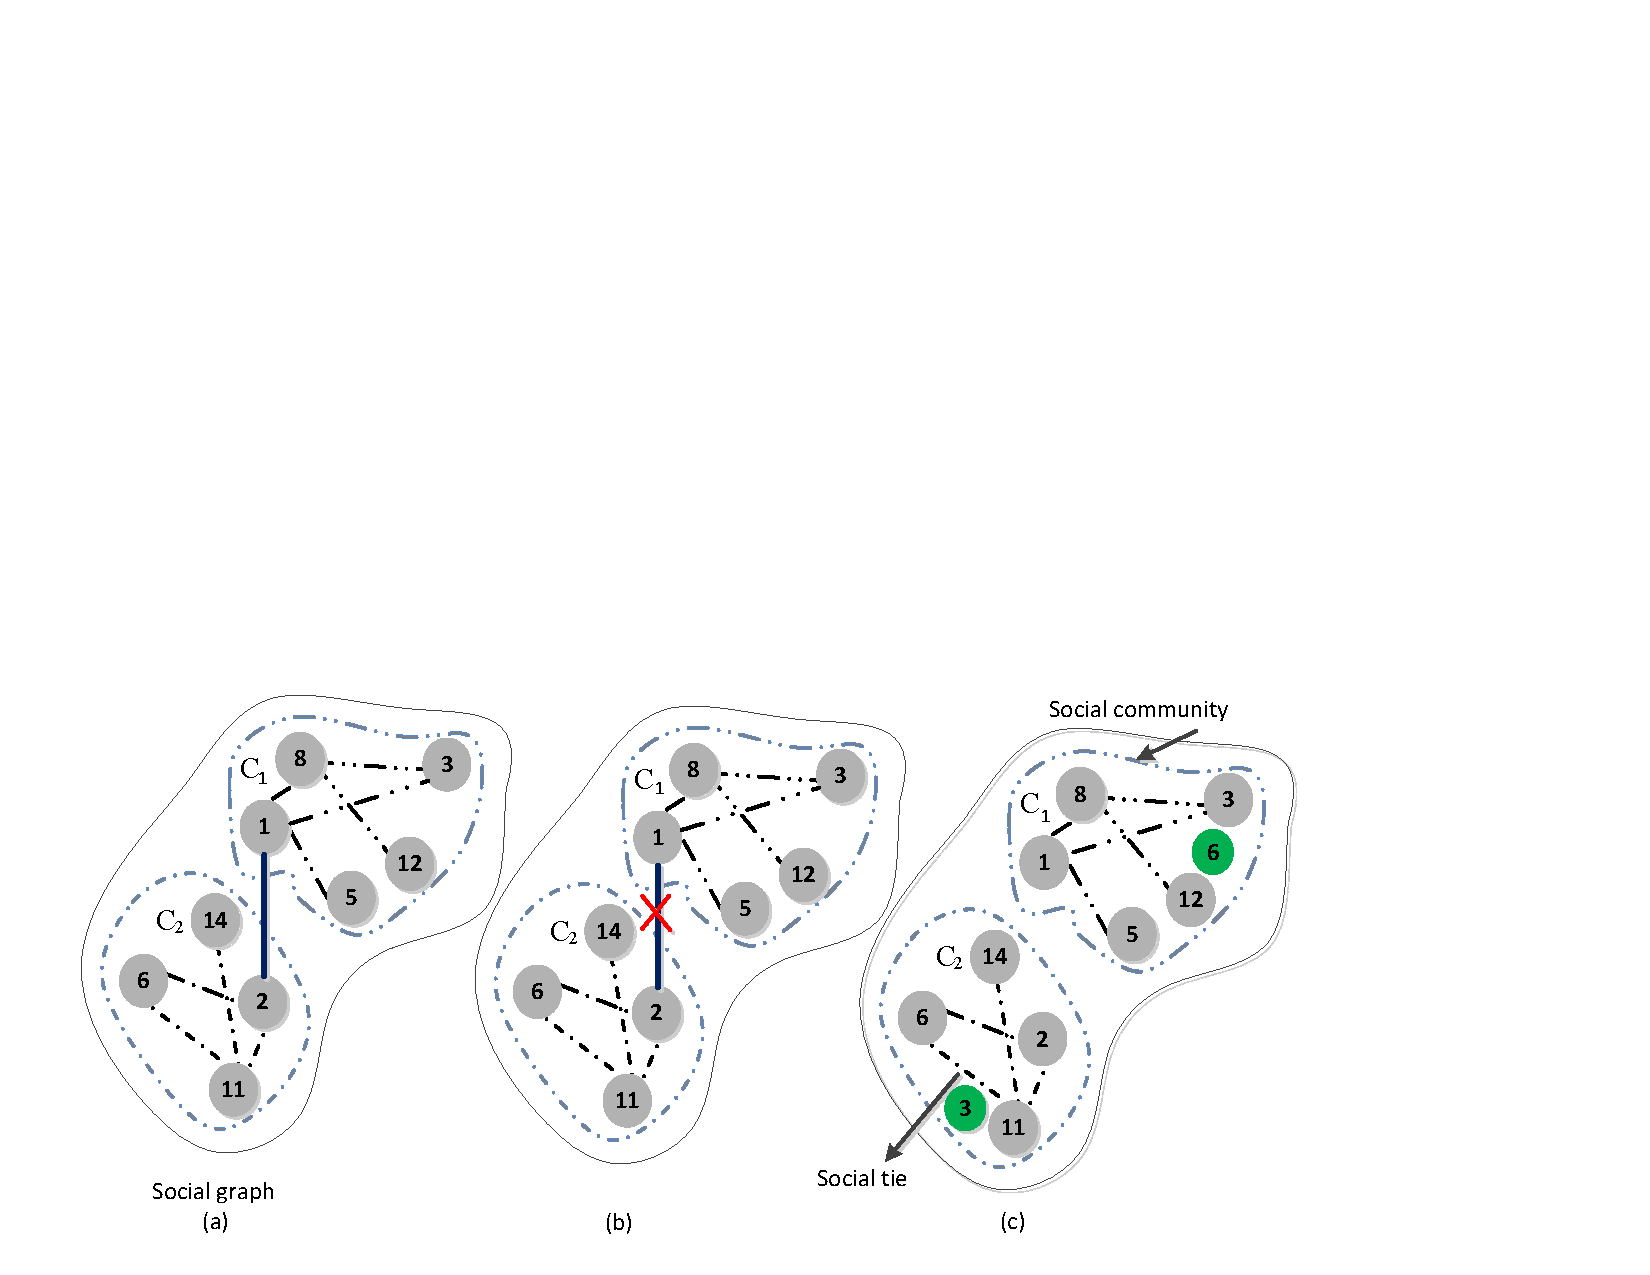
\includegraphics[width=0.8\textwidth]{Chap4-Fig1.pdf}
  \end{tabular}
  \caption{Social graph of ASNETs (C = Community). (a) Distribution of nodes in different communities and data access. (b) Disconnection between the two communities. (C) Community-partition aware data replication example.}
\end{center}
\end{figure}


Primarily there are two different approaches to create copies of data at different nodes: first is replication~\cite{ADerhab2009} and the second is caching~\cite{GXylomenos2012}. Data replication is broadly used to overcome issues originated by community partition which comes from nodes mobility, providing availability and fault-tolerance to data management. Therefore, it appears that data replication is an effective way to improve data accessibility in ad-hoc networks~\cite{WLu2010}\cite{GCao2004}\cite{LDFife2004}. However, it is impossible to replicate all data items on every node because of the limited resources. The question is where and how we should allocate the data replicas to gain high data accessibility and availability.

The problem in ASNETs is that most of the operations are based on the data of a user and neighbors' data. In situations where users belong to more than one community, there is no disjoint partition where users and all its neighbors can be co-located, which causes traffic. The problem becomes particularly acute under random partitioning, which is the {\it de-facto} standard in social networks~\cite{Pujol2010}. On the other hand, replicating user's data in multiple or all the servers eliminates the inter-server traffic for reads but increases the replication overhead. In our case, we assume that; 1) a user belongs only to one community, and 2) created social communities should be determined not only by common interests or contacts but also by mobility-related context~\cite{PBellavista2013}. Hence, nodes collaborate and move as a group instead of individually.

The rest of this chapter is organized as follows. Related work is discussed in~\ref{Chap4_02}. Then,~\ref{Chap4_03} describes overview of our system model. \ref{Chap4_04} explains ComPAS, our replica allocation method. Next, \ref{Chap4_05} presents the performance evaluation result, analysis and discussion. Finally, we summarize the chapter in~\ref{Chap4_06}.

\section{Related Work}\label{Chap4_02}
\esection{Related Work}
Related works falls into three main areas denoted by social-aware, cloud deployment, and socially-oblivious.

Social-aware: This category exploits social properties (friendship, similarity, centrality, etc.) to replicate data. Pujol {\it et al.}~\cite{Pujol2010} have investigated the difficulties of scaling online social networks, and designed a social partitioning and replication middleware in which users' friends can be co-located in the same server.

Cloud deployment: The need for highly scalable and elastic network resources are required to deploy new social applications, it is promising to deploy them in the cloud~\cite{PStuedi2011}\cite{ZWang2012}. When placing social networks data among multiple clouds, it maintains the social locality by replicating the data of a user's every neighbor to the cloud that hosts the user's own data. Maintaining social locality eliminates the inter-cloud multi-get traffic and an unpredictable response time because all the data requested by a user can be retrieved from a single cloud. The RFH~\cite{YQu2012} algorithm employs traffic load evaluation to figure out the nodes that are in the traffic hub, and then the decision on whether to replicate, migrate or suicide is up to every individual distributed virtual node.

Socially-oblivious: While R3~\cite{XTie2011} is an algorithm that can cope with the dynamic nature of nodes and is based on the distribution of path delays, their model ignored integration of social properties and the effects of load. It showed replication yields significant delay gains if and only if the path delays have high unpredictability without making any other assumptions about the underlying delay distribution.

Different from the above mentioned related works; we consider social relationship as a social behavior and user interactions within the community which uses social graph to achieve better data availability after the network division because of the dynamic nature of ASNETs. Most related are the studies by Pujol {\it et al.}, who considered scalability for designing and implementing the social partitioning and replication middleware that transparently leverages the social graph structure to achieve data locality while minimizing replication, by Tara {\it et al.}, who have looked at the social relationship and social locality of third-party applications in Facebook which improves the social network efficiency~\cite{Pujol2010}\cite{DTran2012}. Therefore, ComPAS considers social relationship as a social behavior within the community created from nodes having the same mobility group. It helps to achieve better data availability, consistency and balanced load in the network.

\section{System Model}\label{Chap4_03}
\esection{System Model}
This section describes the social community network, mobility, data management and reliability management models. Further, the theoretical foundation for this system model follows the ASNET middleware framework (Fig. 3.1) proposed in Chapter 3.  The cross-layering approach among the layers and components which will be used as inspiration to build an extended and full-fledged data management middleware. Although, we present the theoretical system model for clarity, notice that this chapter covers and targeted mainly to one of the main technique in data management model called data replication. Hence, we will not necessarily apply all the approaches (i.e., cross-layering, all the models, layers) to the method of replica allocation proposed in this chapter.

\subsection{Social Community Network Model}\label{Chap4_03_01}
\esubsection{Social Community Network Model}
Social network analysis is a useful and powerful tool for analyzing complex social relationships among people in social sciences~\cite{OSerrat2009}. The notion of social network and the methods for social network analysis attract significant interest initially from the social and behavioral communities, later data mining, and only recently from cross-community mining (CCM) proposed by Guo {\it et al.}~\cite{BGuo2012}. Social networks exhibit the small world phenomenon that node encounters are sufficient to build a connected relationship graph. Such a graph is an abstract graph where vertices represent individual people and edges describe social ties between individual people. With a social graph, a variety of social metrics (e.g. social relationship, communality, centrality, and similarity) can be easily calculated and then these metrics can be used by social-based approaches. Therefore, it is crucial to obtain social graphs for social-based data management design approaches like ASNETs.

Community is a structural subunit (which can be represented as a set of individuals) of a social network with high density of internal links. As mentioned in the previous chapters, individuals have more social connections with other individuals inside their own community than with individuals outside. The social connections may be family, friends, common location or common interest, which are decided by the social graph. We assume that the physical network is composed by a set $G$ of $n$ nodes identified by $\{d_0, d_1 ... d_{n-1}, d_n\}$. Every node $d_i \in G$ has a unique address or identification and the same processor and energy capacity. Nodes communicate over a wireless link with a delimited transmission range and its value is the same for all nodes. Nodes move accordingly to a group movement pattern in a surrounded area. Community partitions in the network can occur when the network between the communities fail simultaneously due to movement of nodes or scarce resources. Nodes are assumed to rely on intermediate nodes to route packets since they may not reach all nodes directly due to their coverage area.

\subsection{User Mobility Model}\label{Chap4_03_02}
\esubsection{User Mobility Model}
In reality, the moving behavior of mobile users is usually regular and follows some mobility patterns~\cite{WCPeng2003}\cite{HKWu2001}. Group mobility refers to the scenario where several mobile nodes tend to move together. The system tries to solve the problem of replica allocation by exploring group mobility. The underlying group mobility model is assumed to be Reference Point Group Mobility Model (RPGM). In our system, each mobile node first exchanges its motion behavior with neighbor based on the social relationship in the community. Mobile nodes may collaborate and, hence, move as a group instead of independently. RPGM is proposed in~\cite{JLHuang2006} to model this kind of team collaboration behavior. In RPGM, all mobile nodes are divided into several mobility groups and all mobile nodes within the same mobility group are of similar moving behavior. We assume that each node is equipped with a GPS device and, hence, the position of the node is always available. In our work, we take RPGM as the group mobility model and the movement of each group follows a waypoint model.

\subsection{Data Management (Replica Management) Model}\label{Chap4_03_03}
\esubsection{Data Management (Replica Management) Model}
As mentioned in the previous chapter, data is an important element in all type of networks, particularly in ASNETs. The design techniques that should be considered related to the data management layer of ASNETs from Fig. 3.1 are: data collection and gathering, data dissemination, data processing, data replication and handling~\cite{CSengul2012}. From these techniques the focus of this chapter is on data replication. Replication is a fundamental technique used in distributed systems. Its main aim consists of storing the same data or service at multiple nodes. By replicating data at mobile nodes, data availability can be improved because there are multiple replicas in the network and the probability of finding one copy of the data is high~\cite{ADerhab2009}. Further, data replication can also reduce the query delay, since mobile nodes can get the data replicas from some nearby communities. A replicated object (i.e., replica) is a data item that is stored redundantly at multiple communities. We define data replication as a technique of creating and managing duplicate versions of data items. Each node can perform two types of operations: read and write.

Due to node mobility and dynamic nature of ASNETs, nodes with similar moving behavior (same mobility group) create/form a community. That is, $N$ user nodes with a set of $Y$ communities. $D_{ic}$ = 1 if and only if user $i$'s data is stored at one of the storage space at community $c$, and $\sum_{c=1}^Y D_{ic} = 1 \forall i$.

Our aim in this chapter is to find an efficient and consistent way to store $X$ replicas for each user's data on the storage space at $Y$ communities $(X<Y)$ and we choose the value of $X$ depending on the replication budget of the system and its desired availability or accessibility. Table 4.1 summarizes the notations with their representation or definition we use throughout this chapter.

\begin{table}
\centering
\caption{Definition of Notations/Symbols}
\renewcommand{\arraystretch}{1.5}
\begin{tabular}{|l|l|l|l|l|}
\hline
\multicolumn{1}{c}{Notation/Symbol} & \multicolumn{1}{c}{Definition}\\
\hline
\multicolumn{1}{c}{$D_{ic} = 1$} & \multicolumn{1}{c}{User $i$'s data is stored at one of the storage space of community $c$}\\
\multicolumn{1}{c}{$X$} & \multicolumn{1}{c}{Number of replicas for each user data} \\
\multicolumn{1}{c}{$N$} & \multicolumn{1}{c}{Number of users/nodes} \\
\multicolumn{1}{c}{$r_{ic} = 1$} & \multicolumn{1}{c}{User $i$'s data is replicated at community $c$}\\
\multicolumn{1}{c}{$a_{ij}$} & \multicolumn{1}{c}{Adjacency of two nodes $i$ and $j$ in the social graph}\\
\multicolumn{1}{c}{$a_{ij} = 1$} & \multicolumn{1}{c}{$i$ and $j$ are neighbors (connected directly)}\\
\multicolumn{1}{c}{$RC(i)$} & \multicolumn{1}{c}{Cost of a read query for a user $i$}\\
\multicolumn{1}{c}{$ARC$} & \multicolumn{1}{c}{Average read cost for a user $i$}\\
\multicolumn{1}{c}{$\ell(c)$} & \multicolumn{1}{c}{Load for a storage space $c$}\\
\hline
\end{tabular}
\end{table}

Since we have two types of data queries (read and write), in the remaining part of this section we will formulate or calculate the cost of read/write query for a user $i$.

\subsubsection{Cost of a Read Query for a User $i$}\label{Chap4_03_03_01}
%\esubsubsection{Cost of a Read Query for a User $i$}
Cost of ready query represents the number of communities required to retrieve the data of user $i$ and that of every neighbor of $i$. To retrieve user $i$'s data, the query is sent to its primary/own community, say in community $c$ (i.e., $D_{ic} = 1$), and thereby incurs a cost of 1 (using boolean notation which is 0 and 1).

For each neighbor $j$ of $i$ (i.e., $a_{ij} = 1$), there are three cases as detailed in Algorithm 1 and Fig. 4.2:

\begin{algorithm}
  \Begin{
    For each neighbor $j$ of $i$\;
     \ForAll{$a_{ij} = 1$}{
        \If {$j$'s data is co-located with $i$'s data (i.e., $D_{jc} = 1$)}{
            stay on the same community $c$ to read $j$'s data;
            (no additional cost, read cost = 0)}
        \If{Replica of $j$'s data is co-located with $i$'s data (i.e., $r_{jc} = 1$)}{
            stay on the same community $C$ to read $j$'s data;
            (no additional cost)
        }
        \Else{
            go to $j$'s community to read its data
            (an additional cost of 1, go to a different community)
        }
     }
     $i$ and $j$ are not direct neighbors
}
\caption{Pseudocode of read cost for a user $i$}
\label{alg:chap4_alg01}
\end{algorithm}

\begin{figure}[h]\label{fig:Chap4-Fig02}
\begin{center}
  \begin{tabular}{c}
  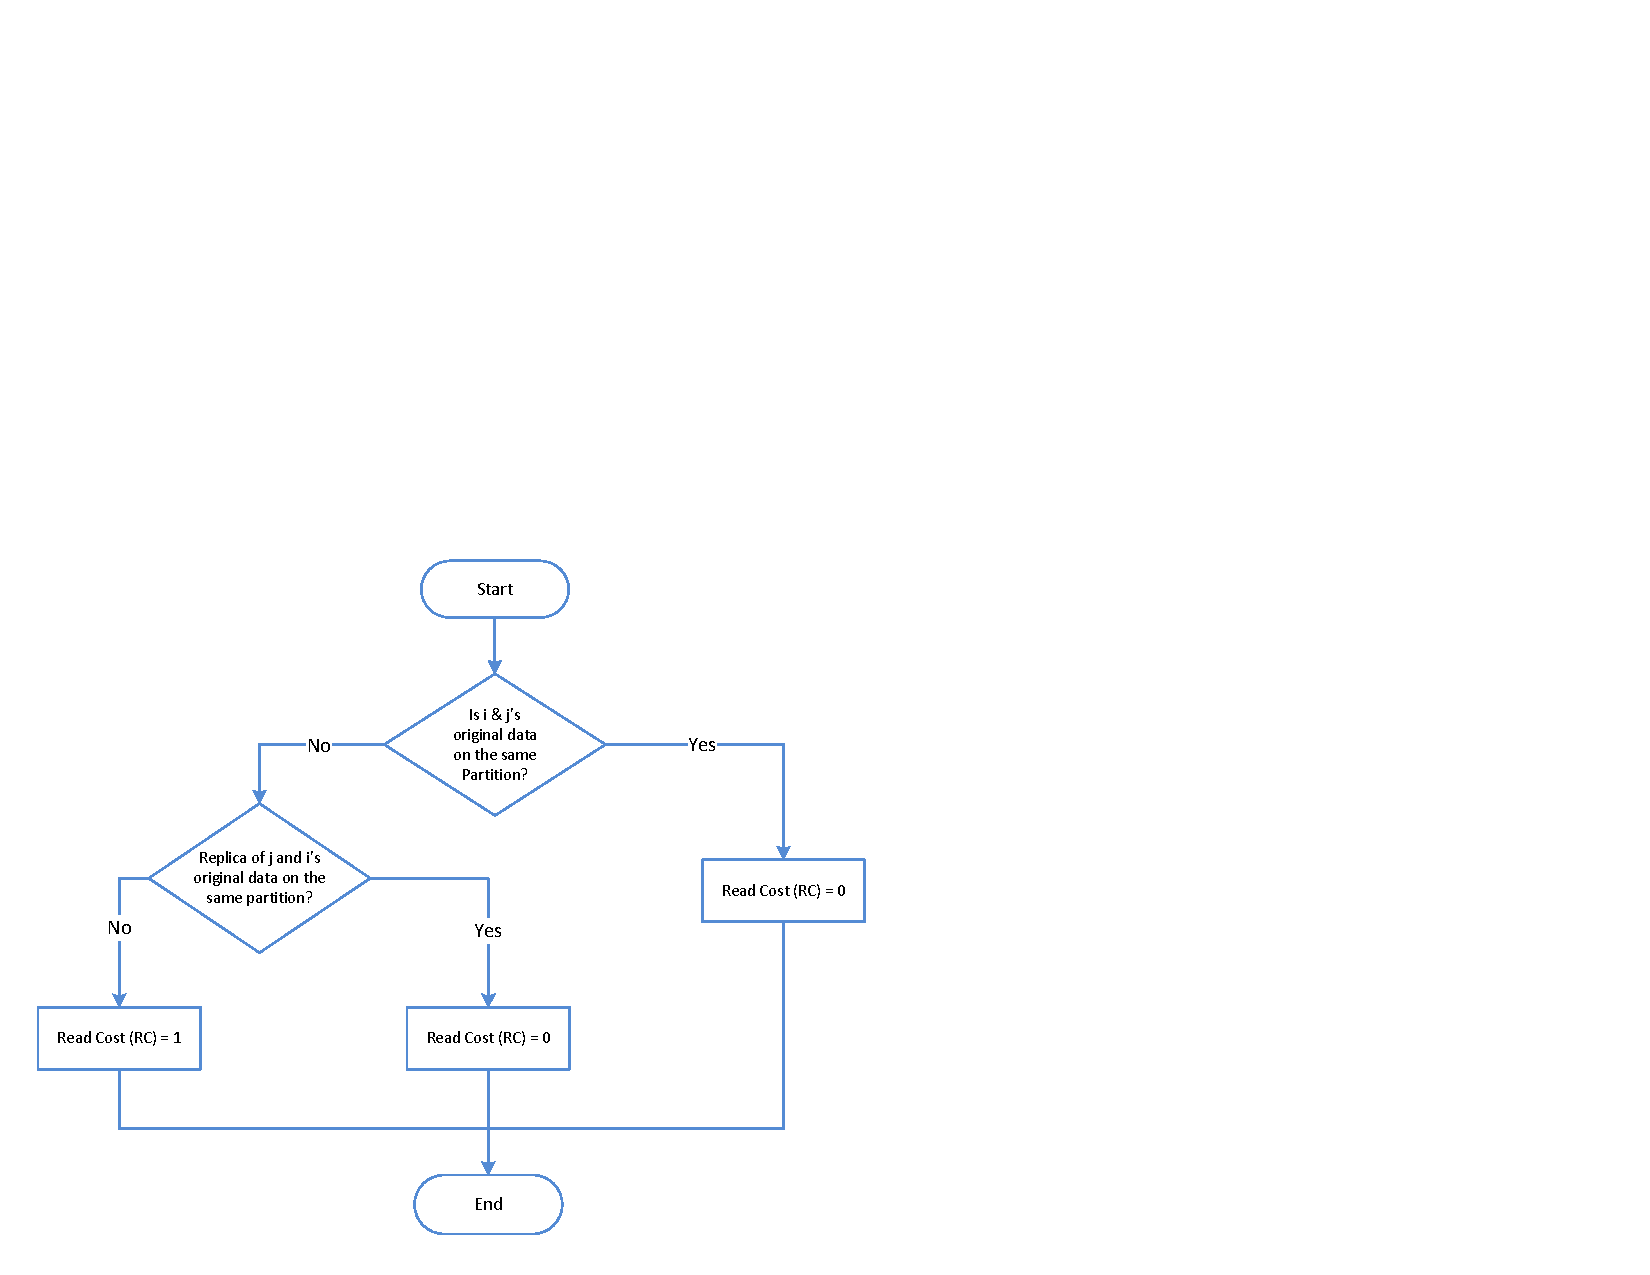
\includegraphics[width=0.8\textwidth]{Chap4-Fig02.pdf}
  \end{tabular}
  \caption{Flowchart for Algorithm 1.}
\end{center}
\end{figure}

Therefore, based on Algorithm 1, a read query by user $i$ incurs the following cost:
\begin{equation}
RC(i)=1+\sum_{j=1}^N a_{ij}\sum_{c=1}^G D_{ic}(1-D_{jc})(1-r_{jc}).
\end{equation}


\subsubsection{Cost of a Write Query for a User $i$}\label{Chap4_03_03_02}
%\esubsubsection{Cost of a Write Query for a User $i$}
The cost of write query is always $X+1$. That means, $X+1$ communities need to update the data for $i$. Since this cost is fixed for all nodes in the community, we measure the efficiency of our replica allocation method only in terms of the read cost for an average user which is formulated as follows.
\begin{eqnarray}
ARC&=&\frac{1}{N}\sum_{i=1}^N RC(i)\nonumber\\
ARC&=&\frac{1}{N}\sum_{i=1}^N \left(1+a_{ij}\sum_{c=1}^G D_{ic}(1-D_{jc})(1-r_{jc})\right).
\end{eqnarray}
By setting $r_{jc} = 0$ for every $j$ and $c$, it is possible to calculate the average read cost of the original data storage space in the community without replication. Finally, one can get the achieved read cost reduction because of using data replication technique.
\begin{equation}
ARC_0=\frac{1}{N}\sum_{i=1}^N \left(1+\sum_{j=1}^N a_{ij}\sum_{c=1}^G D_{ic}(1-D_{jc})\right).
\end{equation}

Taking the constraints, 1) there are $X$ replicas for each user's data, and 2) replica \& original data can't be available on the same community into consideration, it is also possible to maximize the below obtained read cost reduction using BIP (Binary Integer Programming) problem.
\begin{eqnarray}
RCR&=&ARC_0-ARC\nonumber\\
   &=&\left[\frac{1}{N}\sum_{i=1}^N \left(1+\sum_{j=1}^N a_{ij}\sum_{c=1}^G D_{ic}(1-D_{jc})\right)\right]-\left[\frac{1}{N}\sum_{i=1}^N \left(1+a_{ij}\sum_{c=1}^G D_{ic}(1-D_{jc})\right)\right]\nonumber\\
RCR&=&\frac{1}{N}\sum_{i=1}^N\sum_{j=1}^N\sum_{c=1}^G a_{ij}D_{ic}(1-D_{jc})r_{jc}.
\end{eqnarray}

Our proposed replica allocation method, ComPAS, is presented aiming at providing the desired efficiency and consistency as the primary goal and it also tries to balance the community storage space load as the next goal. An effective method to deal with the problem of storage overload is to distribute the load over replica nodes, as this helps to achieve a higher efficiency by reducing storage response latency and the number of hops~\cite{ADerhab2009}\cite{HShen2010}. Therefore, load for a storage space is proportional to the amount of data, original or replica, stored in the same space, and can be represented by:
\begin{equation}
\ell(c)=\sum_{i=1}^N (D_{ic}+r_{ic}).
\end{equation}

In order to decide the most desirable location to place the replica of user $i$'s data, it's necessary here to put the formula for computing the location histogram~\cite{DTran2012}.
\begin{equation}
\jmath_i(c)=\sum_{j=1}^N a_{ij}D_{jc},
\end{equation}
where $\jmath_i(c)$ is the number of $i$'s neighbor nodes who are primarily placed at storage space of community $c$.

\subsection{Reliability Management Model}\label{Chap4_03_04}
\esubsection{Reliability Management Model}
\begin{figure}[h]
\begin{center}
  \begin{tabular}{c}
  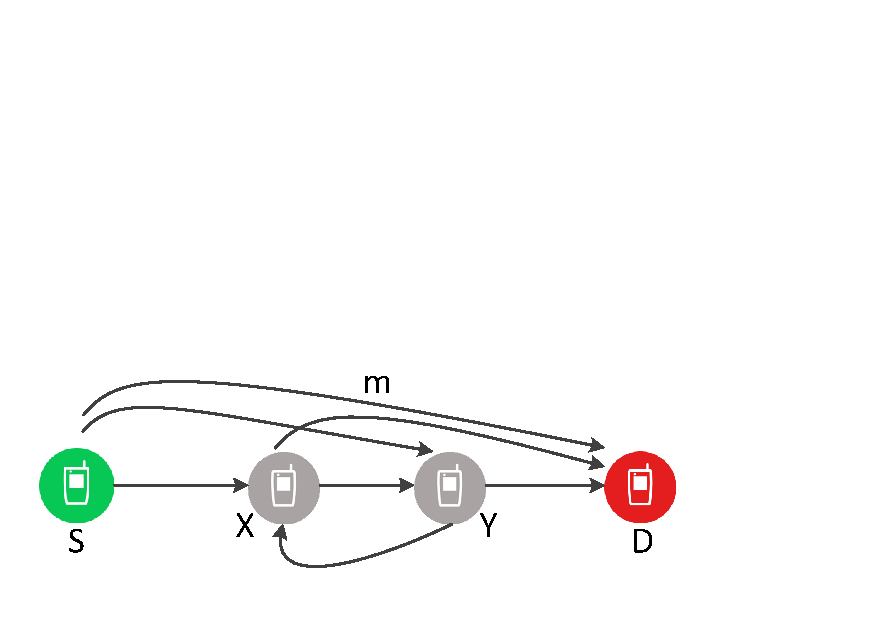
\includegraphics[width=0.45\textwidth]{Chap4-Fig2.pdf}
  \end{tabular}
  \caption{Greedy replica allocation approach example.}
  \label{fig:Chap4-Fig2}
\end{center}
\end{figure}

In our system model, misbehaving nodes compromise the data management by affecting data availability and integrity in a wireless network systems. These nodes are interlopers, and they know how the network works~\cite{YLi2011}. Misbehaving nodes can be either selfish or malicious, or even show both behaviors. Selfish nodes do not collaborate with data management operation, and malicious nodes modify or inject malicious data in the data management system. A misbehaving node is either selfish or malicious throughout its participation in the network and act intermittently. Since ComPAS doesn't exclusively consider reliability, we leave the details as it's out of the scope of this chapter and presented in chapter 6.


\section{The Proposed Method}\label{Chap4_04}
\esection{The Proposed Method}
The concept of replica allocation depends on the choice of different existing approaches. Thus, these approaches can ease the impact of ASNETs connectivity nature and improve data availability ratio. Greedy and controlled replica allocation approaches are the most common ones~\cite{KWei2013}.

\emph{Greedy Replica Allocation:} It is the simplest version of replica allocation, in which nodes generate and forward copies of data to the encountered relay nodes. Here the relay nodes are not all intermediate nodes but those nodes which are chosen to forward messages. Greedy replica allocation is a fast and robust approach, creating a number of replicas that look for the destination concurrently.

For example, suppose that there are four nodes in a network, where node $S$ has a data m destined to node $D$. As shown in Fig~\ref{fig:Chap4-Fig2}, arrows represent the possible flowing direction of data. Since we assume that nodes will not accept the data's that they have received before, there are five possible paths along which data $m$ is transmitted such as:
$S\rightarrow X\rightarrow Y\rightarrow D,~S\rightarrow X\rightarrow D,~S\rightarrow D,~S\rightarrow Y\rightarrow X\rightarrow D$ and $S\rightarrow Y\rightarrow D$.
The probability of successful data forwarding is 50\%. If using the greedy replica allocation approach, the probability of data availability is 78.5\%, which is calculated as $1-(1-0.5)~x~(1-0.5^2)^2~x~(1-0.5^3)^2$. If using other replica allocation approaches, the maximum delivery ratio can be achieved when $S$ directly copy data $m$ to $D$, and the availability ratio is 50\%.
Note that the greedy replica allocation explained above and used for ComPAS is different from the replication way used in epidemic algorithm~\cite{AVahdat2000}. In epidemic, replicas are blindly forwarded to all encountered nodes, resulting in consuming a large number of network resources. However, the greedy replica allocation used here only allows nodes to transmit copies to the storage space which are chosen to store the replicas.
\begin{figure}[h]
\begin{center}
  \begin{tabular}{c}
  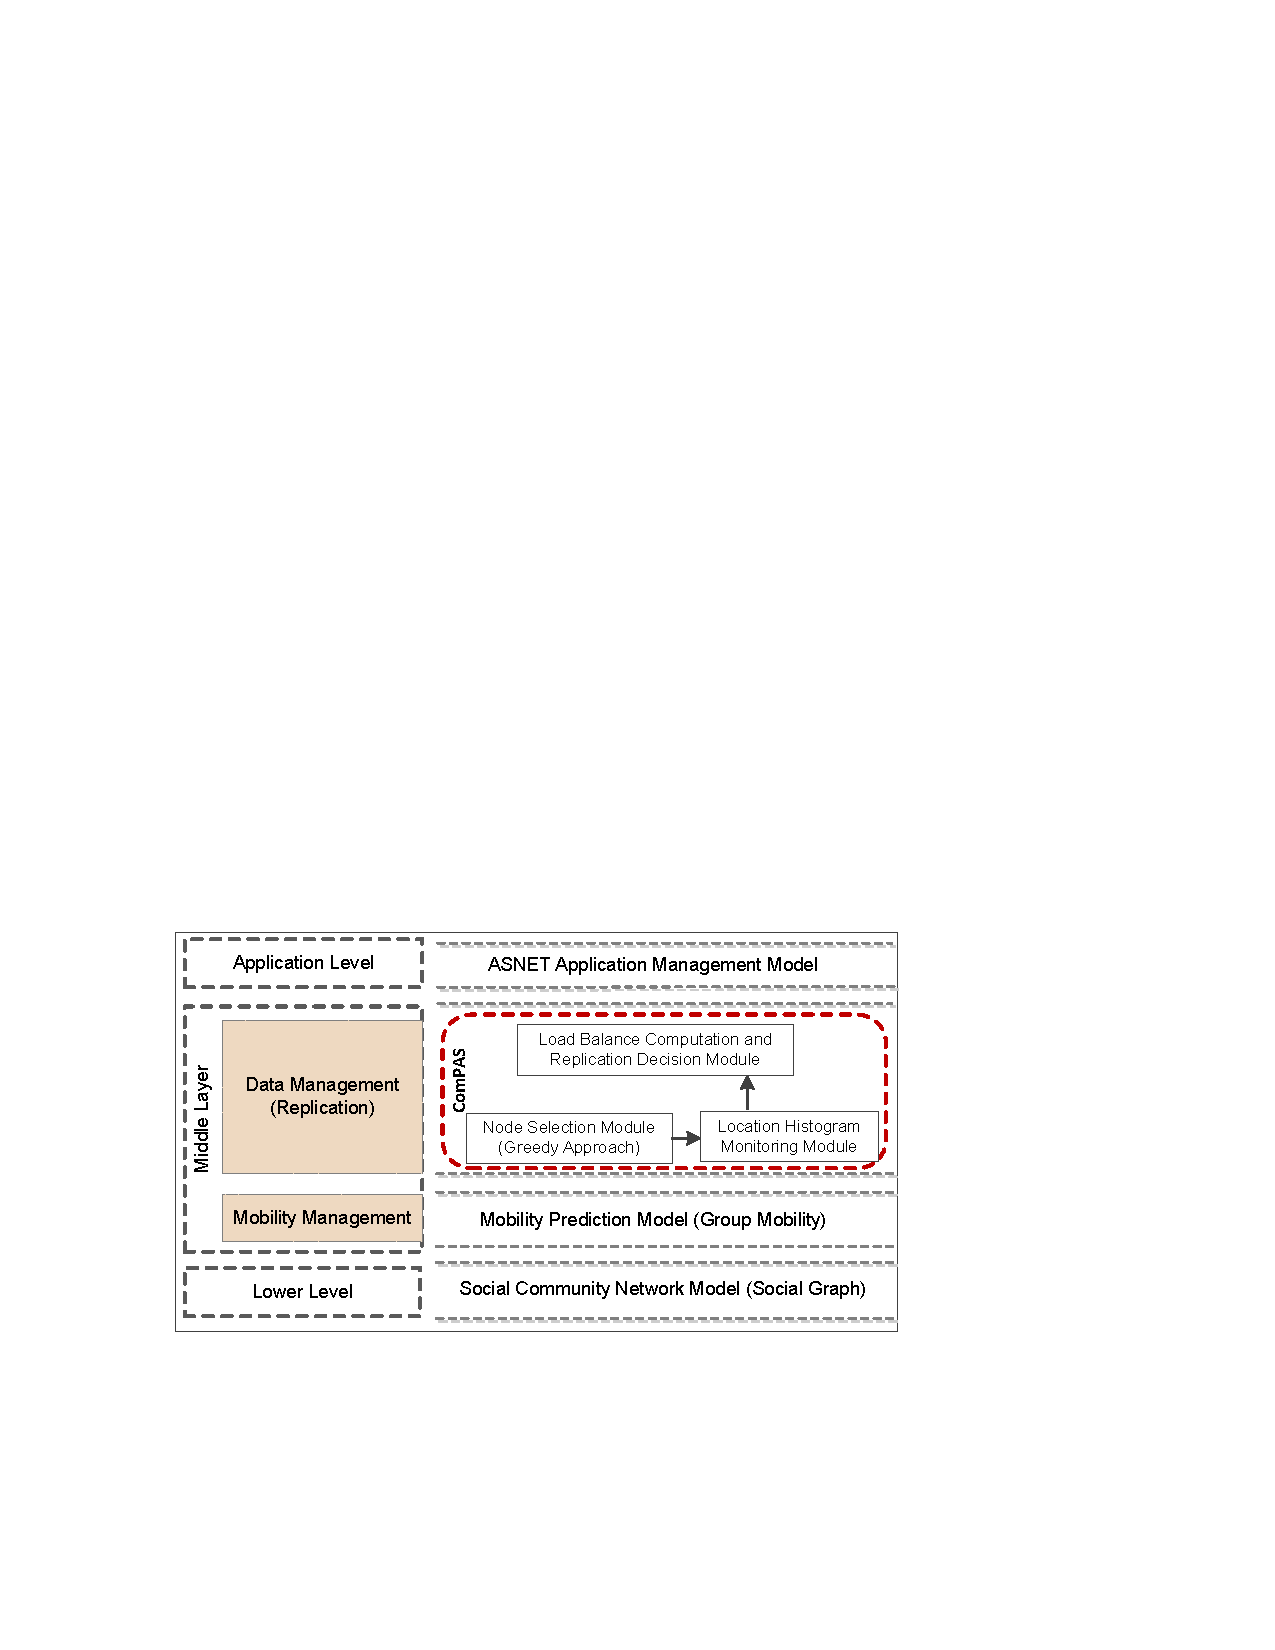
\includegraphics[width=0.68\textwidth]{Chap4-Fig3.pdf}
  \end{tabular}
  \caption{ComPAS System Model.}
  \label{fig:Chap4-Fig3}
\end{center}
\end{figure}

\emph{Controlled Replica Allocation:} Although spreading multiple replicas can increase the number of successful availability of data, it may produce considerably high overhead in terms of buffer space and energy spent on transmission and reception. Deterministic and real-time controlled replica allocations are approaches under this category, which transmit fewer replicas in a network. Encounter based routing~\cite{SCNelson2009} is an example of the real-time controlled replication.

The system model depicted in Fig. 4.4 presents ComPAS's operation and the connection it has with the lower and upper layers.  ComPAS modules (node selection, location histogram, load balance computation and replication decision), the components and layers will be used as an inspiration to build an extended and full-fledged data management middleware. Initially, there is a social network which have a number of communities. We need to create/generate a social graph of that social network using RPGM. When community partitioning occurs, there is a need to have a copy/replica of nodes in communities that doesn't contain the primary data. To conduct that, the three steps in the ComPAS model are important. The three steps are demonstrated with the two algorithms (Algorithm 1 and 2). ComPAS is based on a perception that if we need to place a replica copy for a user $i$ somewhere, the most desirable location should be the primary storage place of most neighbors of $i$; this way, most neighbors will benefit from this replica when they issue a read query. The figure illustrates the interaction among the modules of ComPAS which is detailed in Algorithm 2 and the models at the layer level including application management model.

\begin{algorithm}
\Begin{
    {\underline{Notice:}}\\
    The algorithm sequentially considers a node at a time\;
    It uses greedy replica allocation approach for that\;
    Assume that the nodes are processed in the order of ${1, 2, . . . , N}$\;
     \ForAll{$D_{ic} = 1$}{
        compute the location histogram $\jmath_i(c)=\sum_{j=1}^N a_{ij}D_{jc}$ for i (Equation 4.6)\;
        choose the top X storage space of the community c\;
        \If{the storage space has highest $\jmath$}{
            place a replica for user $i$;
        }
        \If{there is a tie [X storage places have the same $\jmath$]}{
            compute $\ell(c)=\sum_{i=1}^N (D_{ic}+R_{ic})$ (Equation 4.5)\;
            choose the storage with least load to place replica for user $i$.
            }
        \Else{
               not enough X storage spaces in the histogram\;
               place it on the storage space with the least load.
        }
    }
}
\caption{Pseudocode of replica allocation}
\label{alg:chap4_alg02}
\end{algorithm}

In order to illustrate ComPAS's basic operation, we presented a network composed of 14 nodes. We are given a social data graph and need to replicate its user data which have been partitioned across the storage space of the community. This case applies an ASNET in its early stage where the network size is considered small (small-scale networks). As an example, we compare ComPAS to full replication and random replication methods when they are applied to a 14 node social graph shown in Fig. 4.5(a). We assume an existing distribution of nodes across three storage spaces $S_1$, $S_2$, and $S_3$ prior to the community partition due to mobility and dynamic nature of ASNETs as shown in Fig. 4.5(b). The movement of nodes in a group creates the formation shown in Fig 4.7.

\begin{figure}[h]
\begin{center}
  \begin{tabular}{c}
  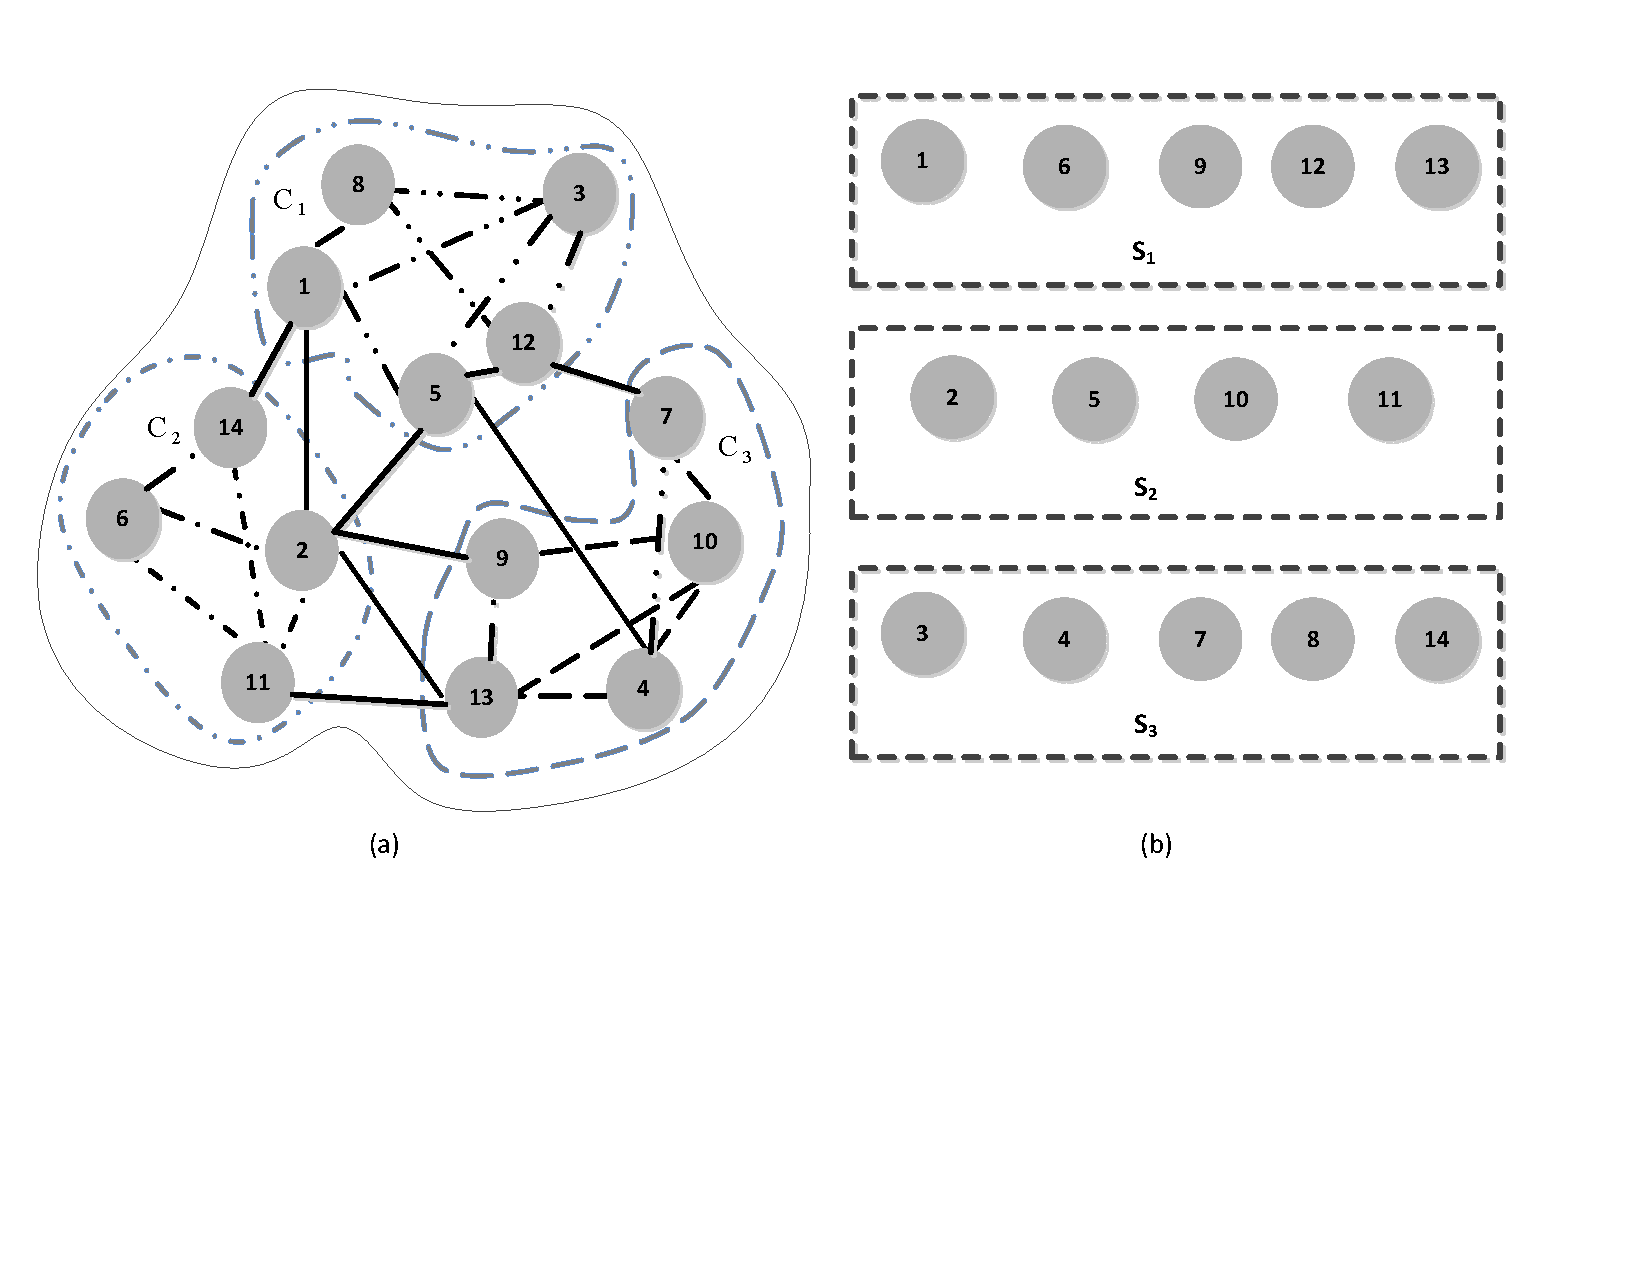
\includegraphics[width=0.7\textwidth]{Chap4-Fig4.pdf}
  \end{tabular}
  \caption{(a) Given Social Graph with 14 nodes and (b) its primary partition of 3 storage spaces.}
\end{center}
\end{figure}

As an example, starting with Node 6, $S_1$ is the primary storage space for it and $S_2$ is the primary storage space for two neighbor nodes of 6 (Nodes 2 and 11) and $S_3$ is the primary storage space for only one neighbor (Node 14). Therefore, $S_2$ is chosen to replicate Node 6 according to Algorithm 2.  The remaining 13 nodes are replicated similarly. The replica allocation operation on the 14 nodes social graph is shown in Fig. 4.6, including the details of who is having a social relationship with who, while calculating the read cost using the formula given in Equation 4.1. After the social graph in Fig. 4.5(a) goes through community-partitioning because of mobility and dynamic nature of the network, it forms the formation shown in Fig. 4.7. It shows the comparison of full replication, random replication and the proposed replication method (ComPAS) with a social relationship of 14 nodes.

\begin{figure}[!t]
\begin{center}
  \begin{tabular}{c}
  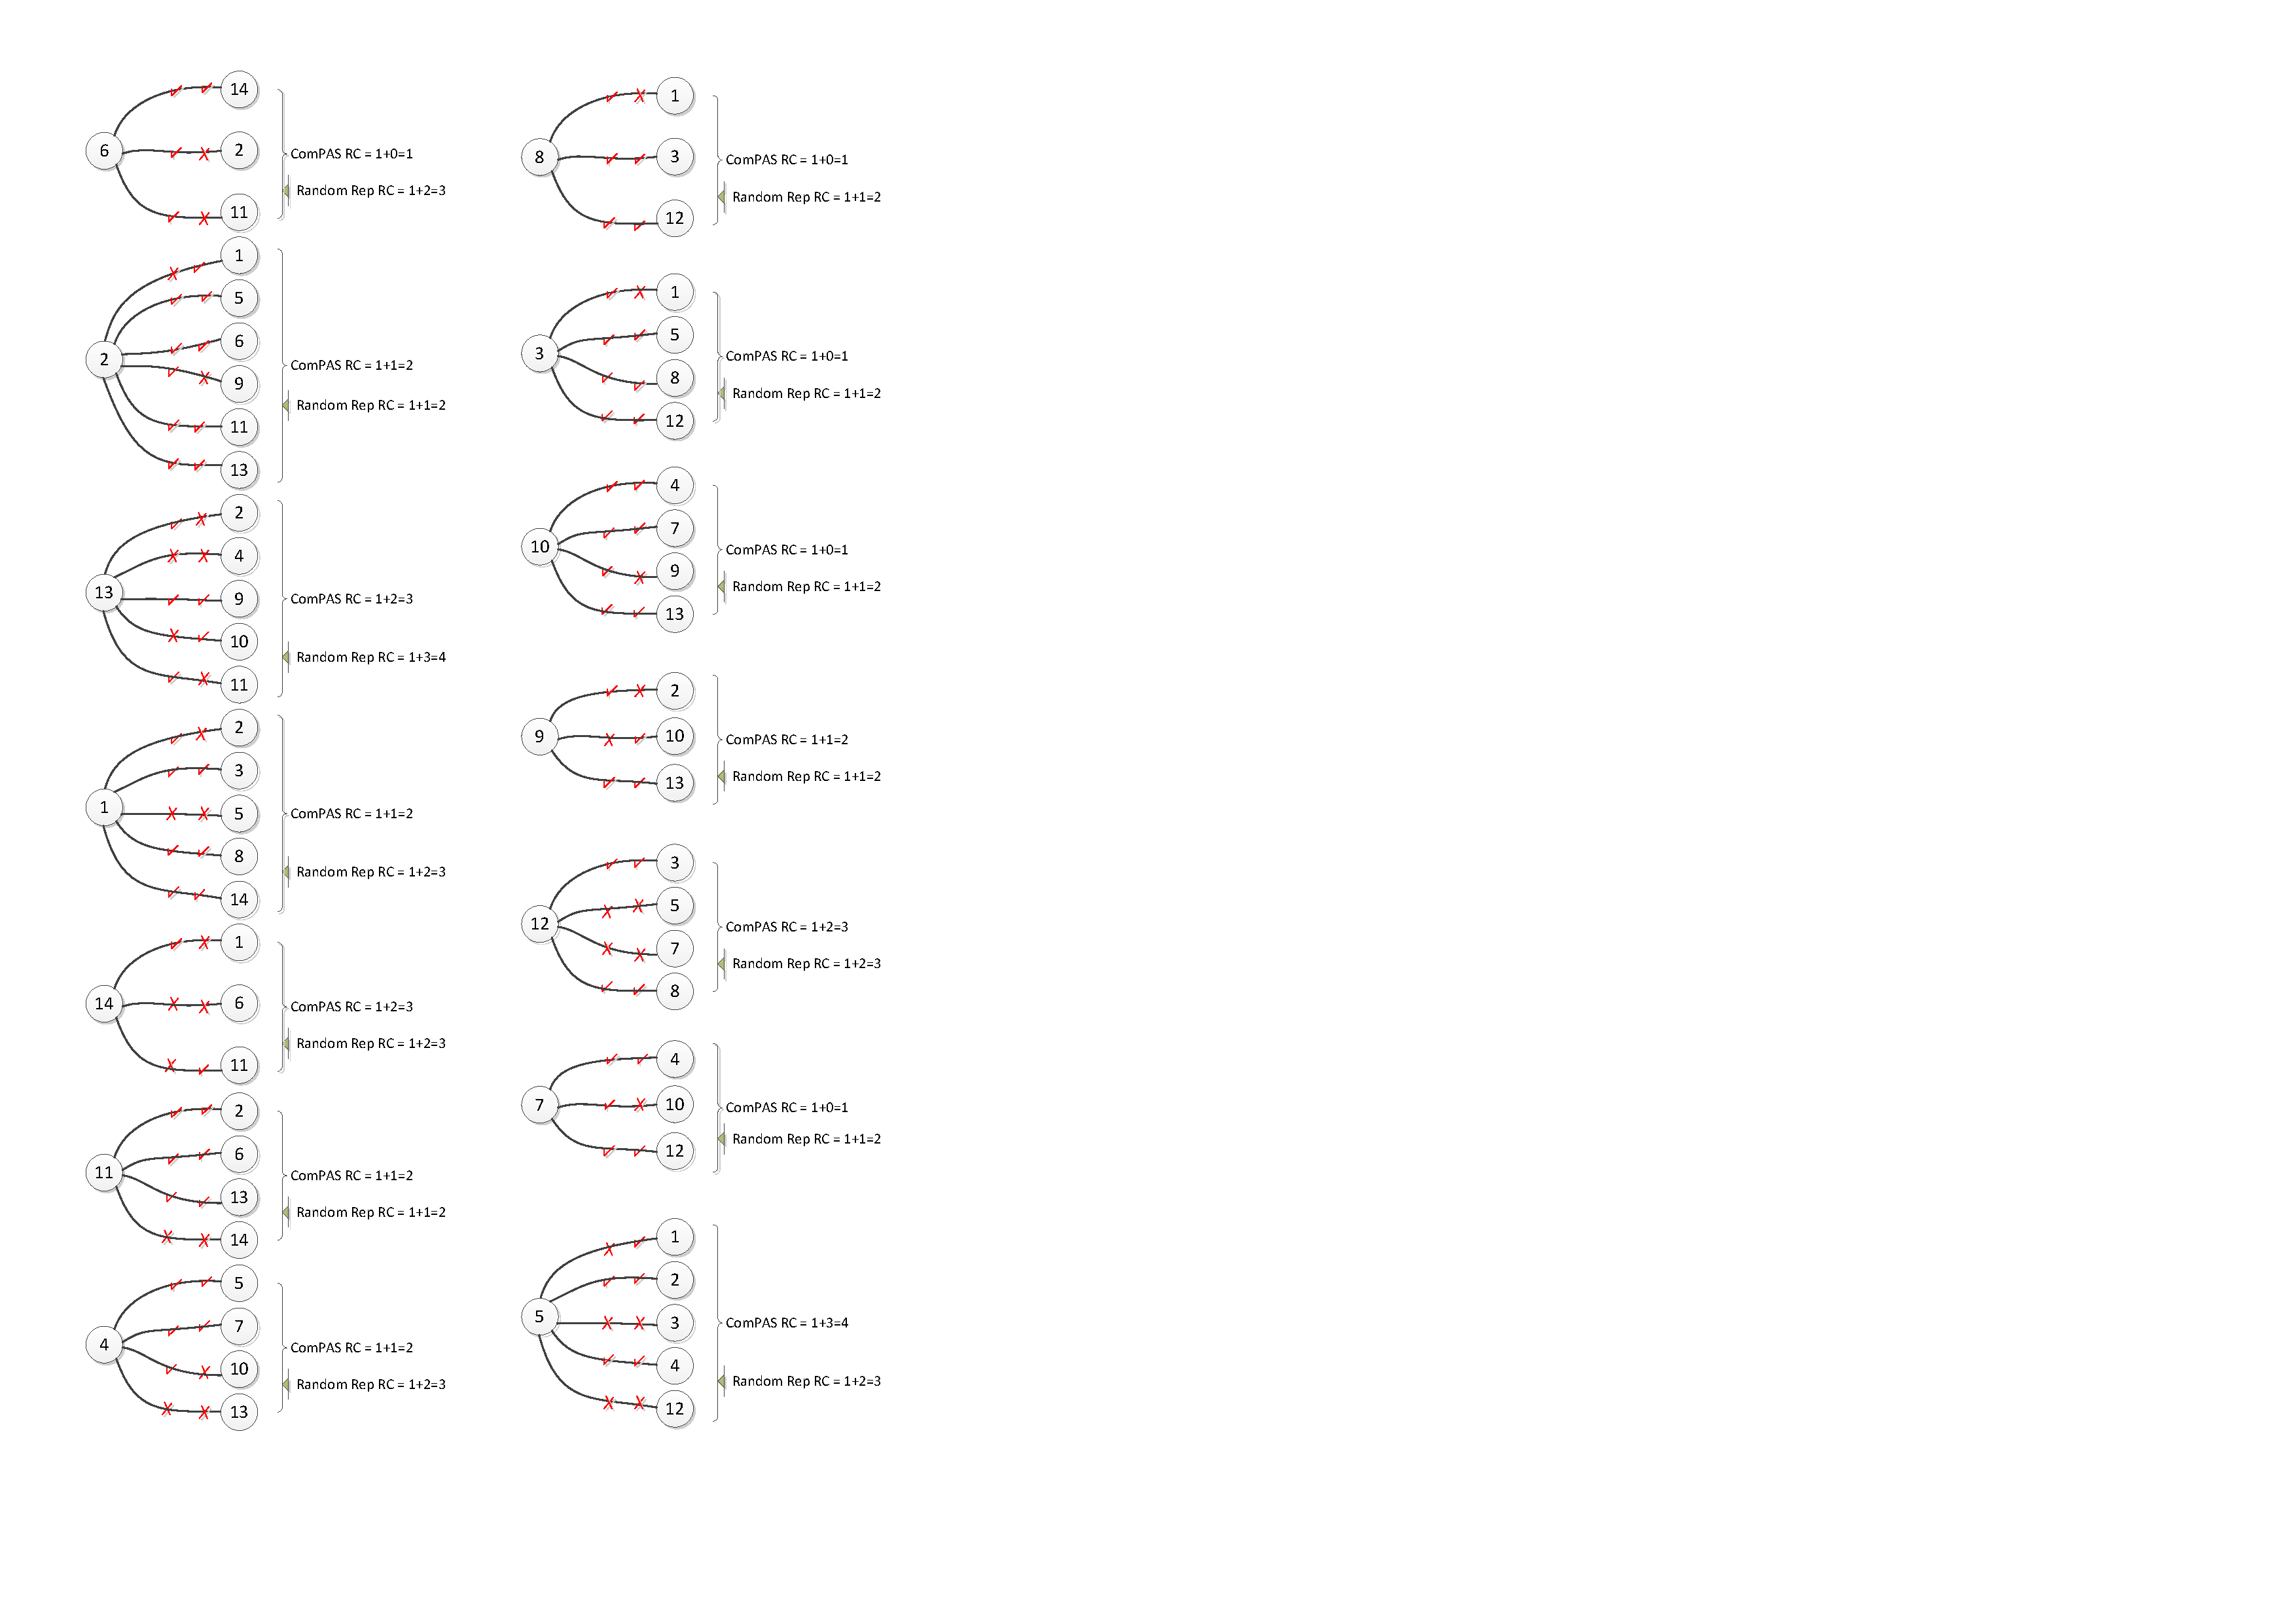
\includegraphics[width=0.75\textwidth]{Chap4-Fig5.pdf}
  \end{tabular}
  \caption{Read cost calculation trace for the 14 node social graph after community-partitioning. (The \checkmark~and $X$ sign on the link indicates a read cost of 0 and 1 respectively. Read cost incurred by ComPAS is represented in the first pattern of each link while the next one is for random replication).}
\end{center}
\end{figure}


From the trace on Fig. 4.6, the total read cost for ComPAS and random replication is 28 and 36, respectively. Therefore, the cost to read the data for each of the 14 users shows a noticeable improvement of ComPAS over random replication (Fig. 4.7(b)) methods, which is about 22.3\% better. Another widely used approach is full replication (Fig. 4.7(a)). In this case, network read traffic falls to 0, but the storage requirements are high (14 units). Full replication also results in high write traffic to maintain consistency. Our proposed solution, ComPAS (Fig. 4.7(c)), performs the best overall.

\begin{figure}[h]
\begin{center}
  \begin{tabular}{c}
  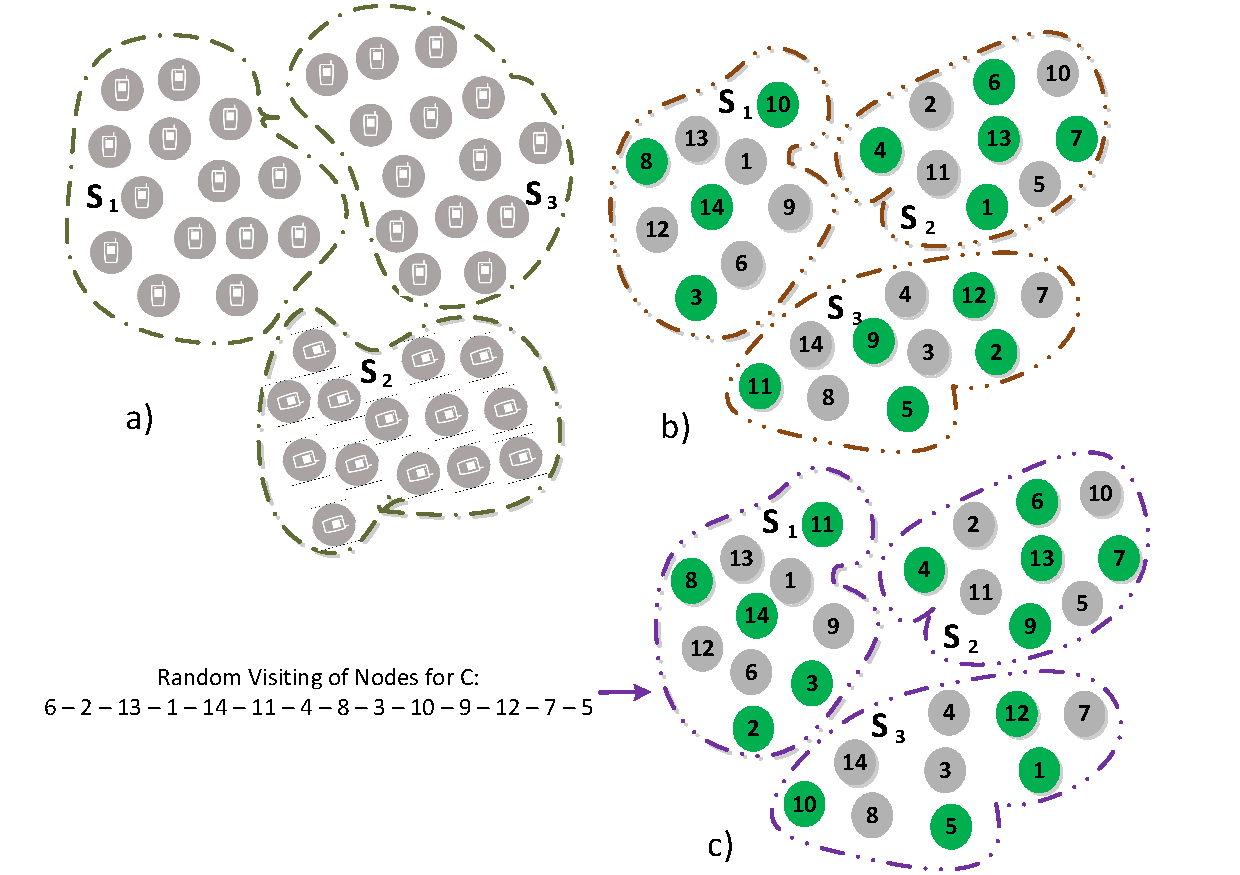
\includegraphics[width=0.8\textwidth]{Chap4-Fig6.pdf}
  \end{tabular}
  \caption{Social graph showing distribution of 14 nodes in 3 communities after partitioning (group mobility pattern).}
\end{center}
\end{figure}

After all the nodes are replicated as shown in Fig. 4.7, we can explain the read cost calculation procedure. \\
\\
\emph{Example 1: Node 6}\\
Node 6 has a direct connection (friendship) with nodes 2, 11, and 14 as shown in Fig. 4.5(a). The primary partition of Node 6 is $S_1$ (with 1, 9, 12, and 13).
To calculate the read cost for Node 6, we use the flowchart depicted in Fig. 4.2 or Algorithm 1. Let's calculate for all the neighbors of Node 6 one by one.\\
{\it Node 6 and Node 2}\\
Case 1: Are the original data of Node 6 and Node 2 on the same partition? As shown above in Fig. 4.5(b), Node 6 belongs to $S_1$ and Node 2 belongs to $S_2$. Therefore the answer is No. We continue to the next case.
Case 2: Are replica of Node 2 and Node 6's original on the same partition? From $S_1$ as shown in Fig. 4.7(c), it is true that primary data of Node 6 and replica of Node 2 are on the same partition. Therefore, the answer is Yes, which means the read cost is 0 according to Algorithm 1.\\
{\it Node 6 and Node 11}\\
Case 1: Are the original data of Node 6 and Node 11 on the same partition? As shown above in Fig 4.5(b), Node 6 belongs to $S_1$ and Node 11 belongs to $S_2$. Therefore the answer is No. We continue to the next case.
Case 2: Are replica of Node 11 and Node 6's original on the same partition? From $S_1$ as shown in Fig. 4.7(c), it is true that primary data of Node 6 and replica of Node 11 are on the same partition. Therefore, the answer is Yes, which means the read cost is 0 according to Algorithm 1.\\ \\
{\it Node 6 and Node 12}\\
Case 1: Are the original data of Node 6 and Node 12 on the same partition? As shown above in Fig. 4.5(b), Node 6 belongs to $S_1$ and Node 12 belongs to $S_1$. Therefore the answer is Yes, which means the read cost is 0 according to Algorithm 1.
Finally the read cost for Node 6 is 1 (the query is sent to its primary/own community) + 0 (Node 2) + 0 (Node 1) + 0 (Node 12) = 1+0+0+0 = 1 as shown in Fig 4.6.

\section{Performance Evaluations}\label{Chap4_05}
\esection{Performance Evaluations}
\begin{figure}[h]
\begin{center}
  \begin{tabular}{c}
  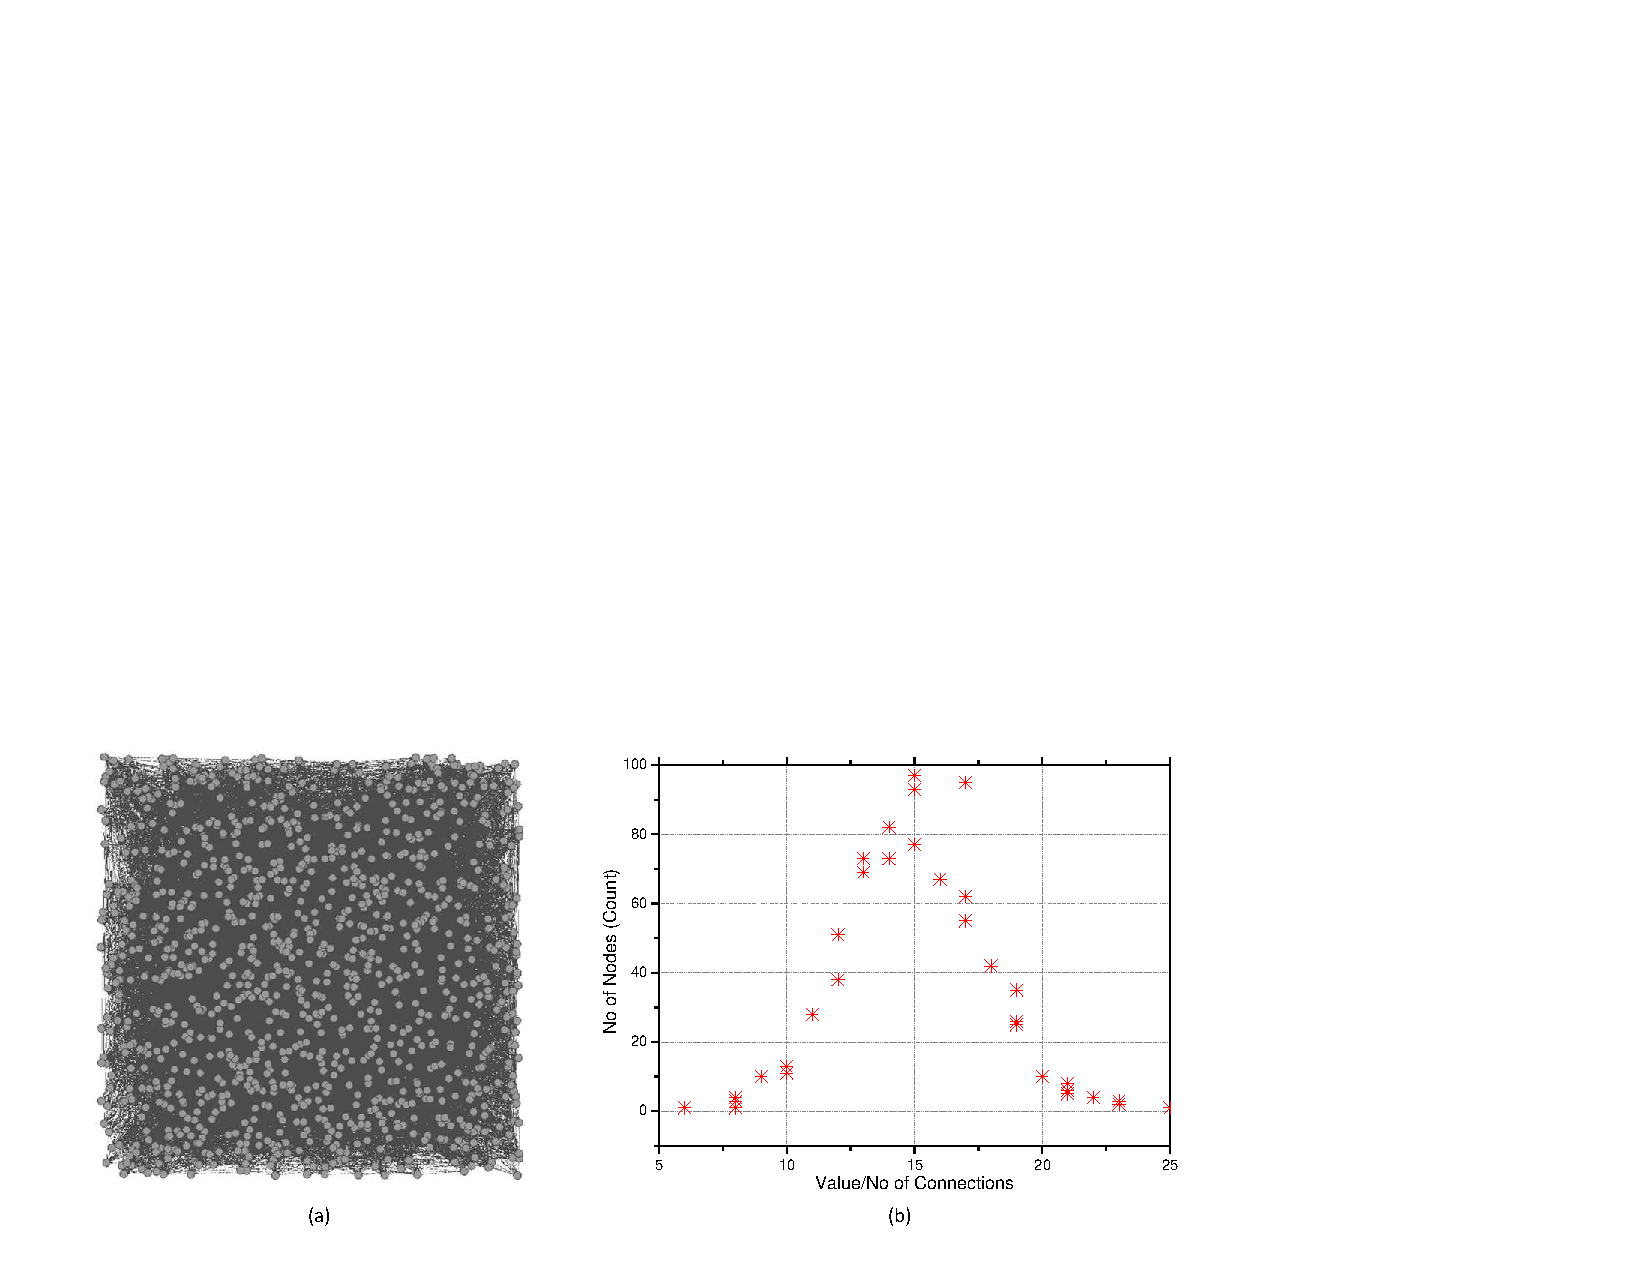
\includegraphics[width=0.9\textwidth]{Chap4-Ev-Fig0.pdf}
  \end{tabular}
  \caption{Evaluation environment (a) a social graph of 1200 nodes, with 17900 edges and average degree of 15. (b) social relationship/degree distribution showing the friendship/direct neighbor.}
\end{center}
\end{figure}

In this section, we evaluate the performance of ComPAS. There is lack of available datasets due to increasing difficulty of crawling social networks. In order to circumvent this, we created synthetic social graph to mimic the structure of social graph using RPGM. we used our own created synthetic social graph consisting of 1200 nodes, 17900 number of links/edges and average degree of 15 as depicted in Fig. 4.8 using the well-known Gephi model\footnote{Gephi is an open-source software for visualizing and analyzing large networks graphs (http://gephi.org/).}. The graph we created does not represent any specific social network in the real world, but it can be used to generate and evaluate small-scale networks. The performance of the new ComPAS data replica allocation method has been compared with the data lookup using an underlying ad-hoc replication protocol (no-replication), random replication scheme and the data replication approach W-DCG as given in~\cite{SJain2013}. In our evaluation, the range for the number of storage spaces is $G \in \{4,8,12,16\}$, and for the number of replicas, $X \in \{1,3,5,...,G-1\}$. The performance of ComPAS has been analyzed and compared with the above three protocols in terms of the metrics collected for our analysis as presented below:

\subsection{Read Cost}\label{Chap4_05_01}
\esubsection{Read Cost}

\begin{figure}[h]
\begin{center}
  \begin{tabular}{c}
  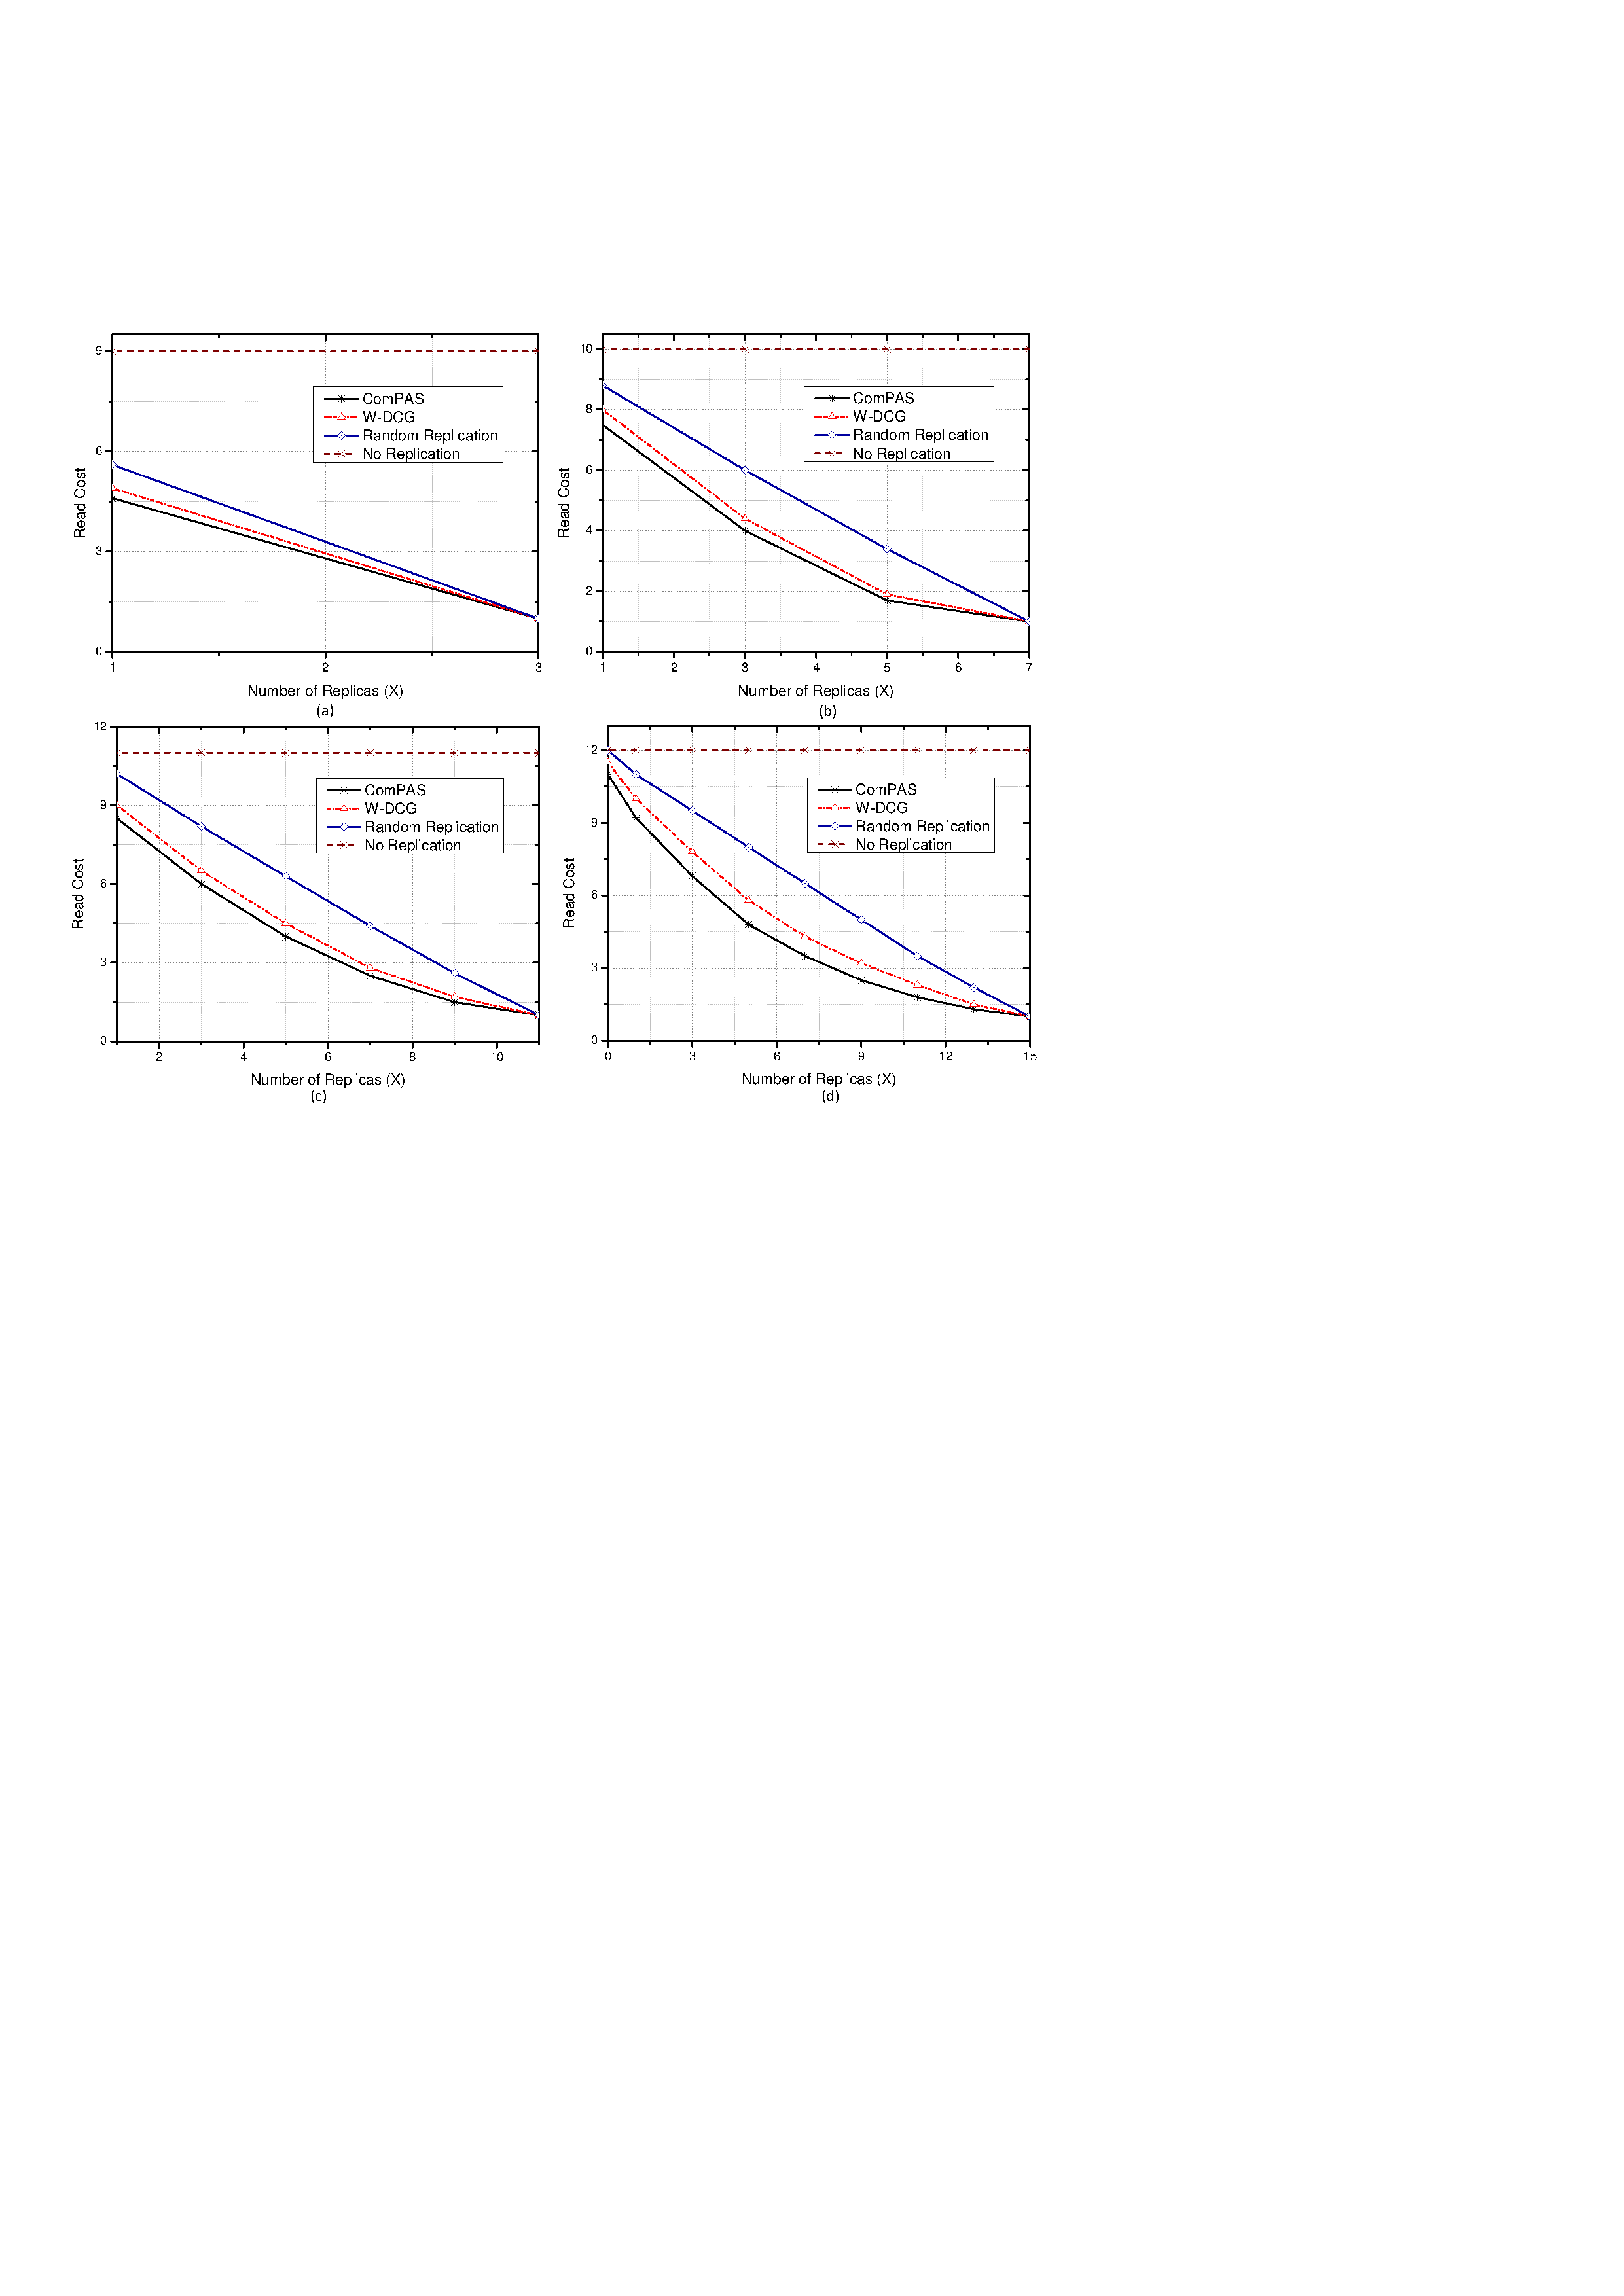
\includegraphics[width=0.95\textwidth]{Chap4-Ev-Fig1.pdf}
  \end{tabular}
  \caption{Replication efficiency in terms of read cost (no replication, random replication, W-DCG and ComPAS).}
\end{center}
\end{figure}

As seen in Fig. 4.9, without any replication, an average read cost is about nine storage space reads per user when the number of storage space is four. This cost increases slowly as more storage spaces are deployed, to a cost of about 12 when there are 16 storage spaces. The read cost improves with replication. However, the improvement of random replication is linear as more replicas are stored. W-DCG's efficiency lowers when compared to the proposed one as the numbers of replicas are increasing. Therefore, it's evident that ComPAS offers a more interesting pattern. Comparing to random replication and W-DCG in terms of replication efficiency, the proposed method is the obvious superior scheme, especially when the number of storage space is increased. Another observation from Figs. 4.9(a)-(d) is that, for each given $G$, there is a value for $X$ that maximizes the efficiency gap among the proposed one, random replication and W-DCG. Almost similar results regarding the replication efficiency of the proposed one, random replication and W-DCG are observed with all the graphs in Fig. 4.9.


\subsection{Data Accessibility and Traffic}\label{Chap4_05_02}
\esubsection{Data Accessibility and Traffic}
\begin{figure}[h]
\begin{center}
  \begin{tabular}{c}
  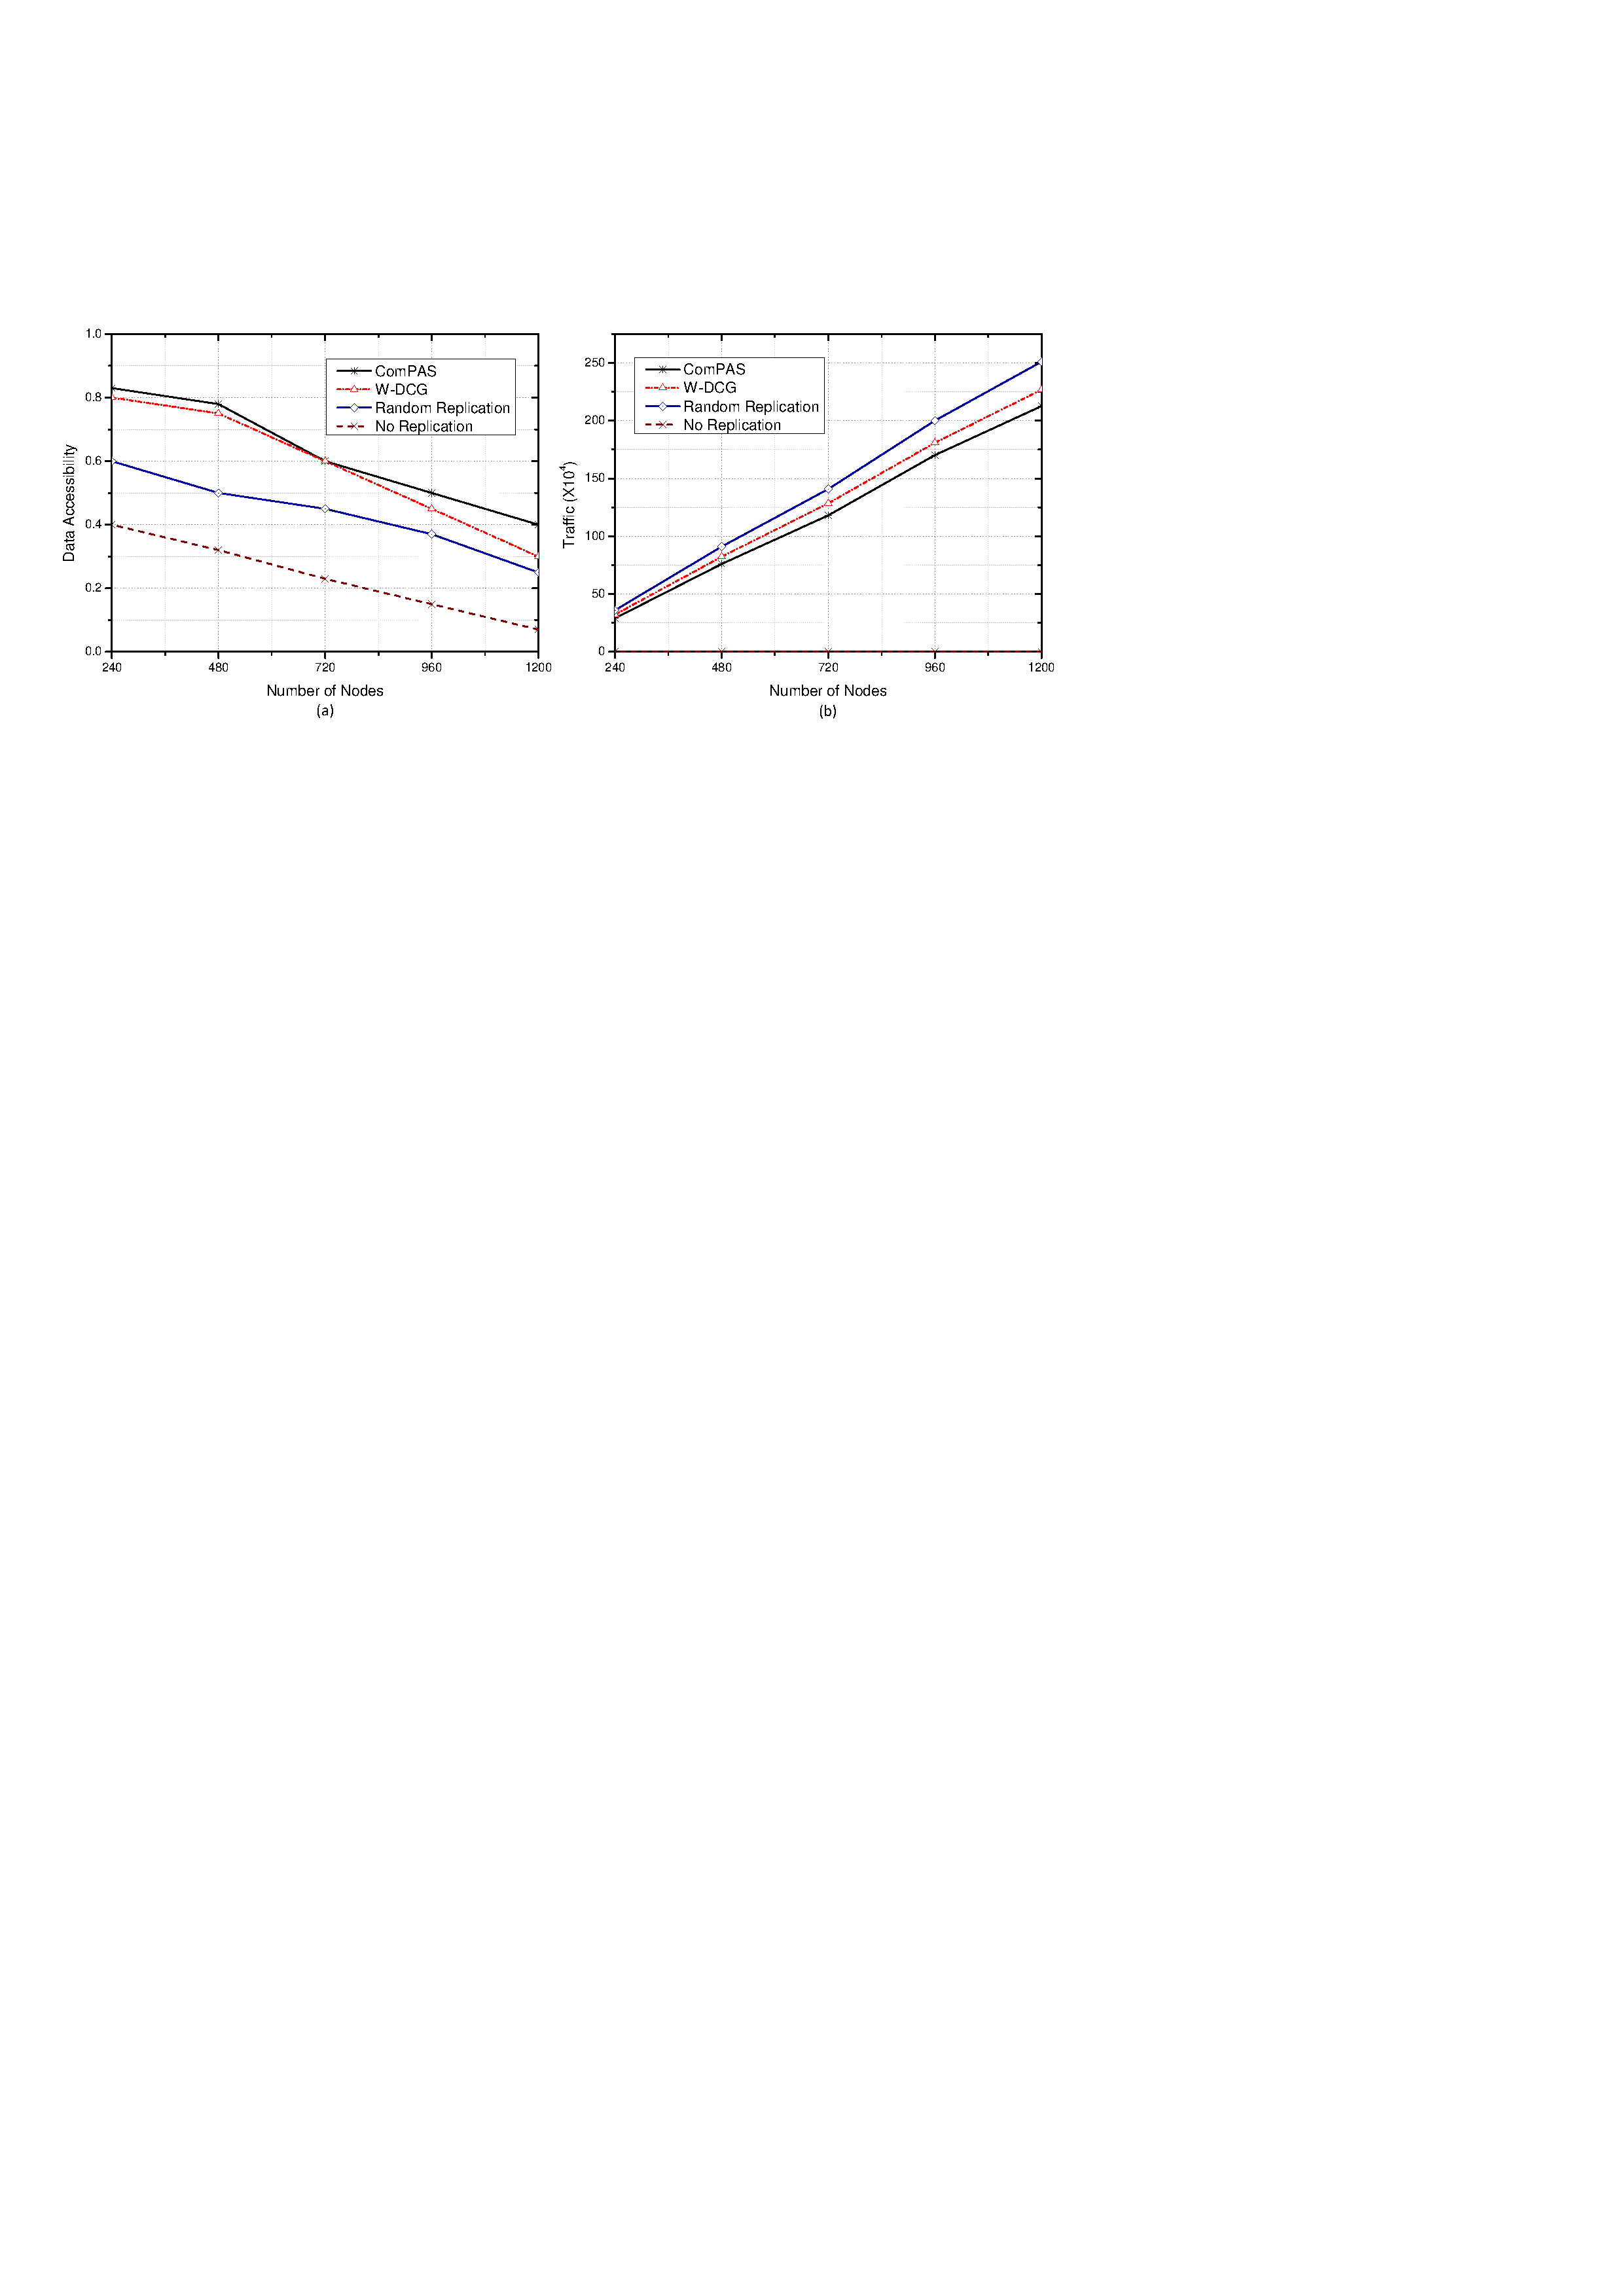
\includegraphics[width=0.95\textwidth]{Chap4-Ev-Fig2.pdf}
  \end{tabular}
  \caption{Effect of number of nodes on (a) data accessibility and (b) network traffic.}
\end{center}
\end{figure}

This is an important criterion for a replication protocol. Basically, data accessibility is the ratio of the number of successful access requests to the number of all access requests issued. A data replication protocol aims to increase the accessibility of data items in the network. Different than conventional static networks, in ASNETs achieving 100\% data accessibility is nearly impossible, due to mobility of nodes and changing network topology. Fig. 4.10(a) shows the variation of data accessibility with varying number of nodes in all the four replication methods including ours. As the number of nodes increases, the number of data items to be replicated in the network also increases, hence the data accessibility reduces. The graph in Fig. 4.10(a) illustrates that ComPAS provides slightly higher data accessibility than W-DCG and higher accessibility than random replication and without replication.
\begin{figure}[h]
\begin{center}
  \begin{tabular}{c}
  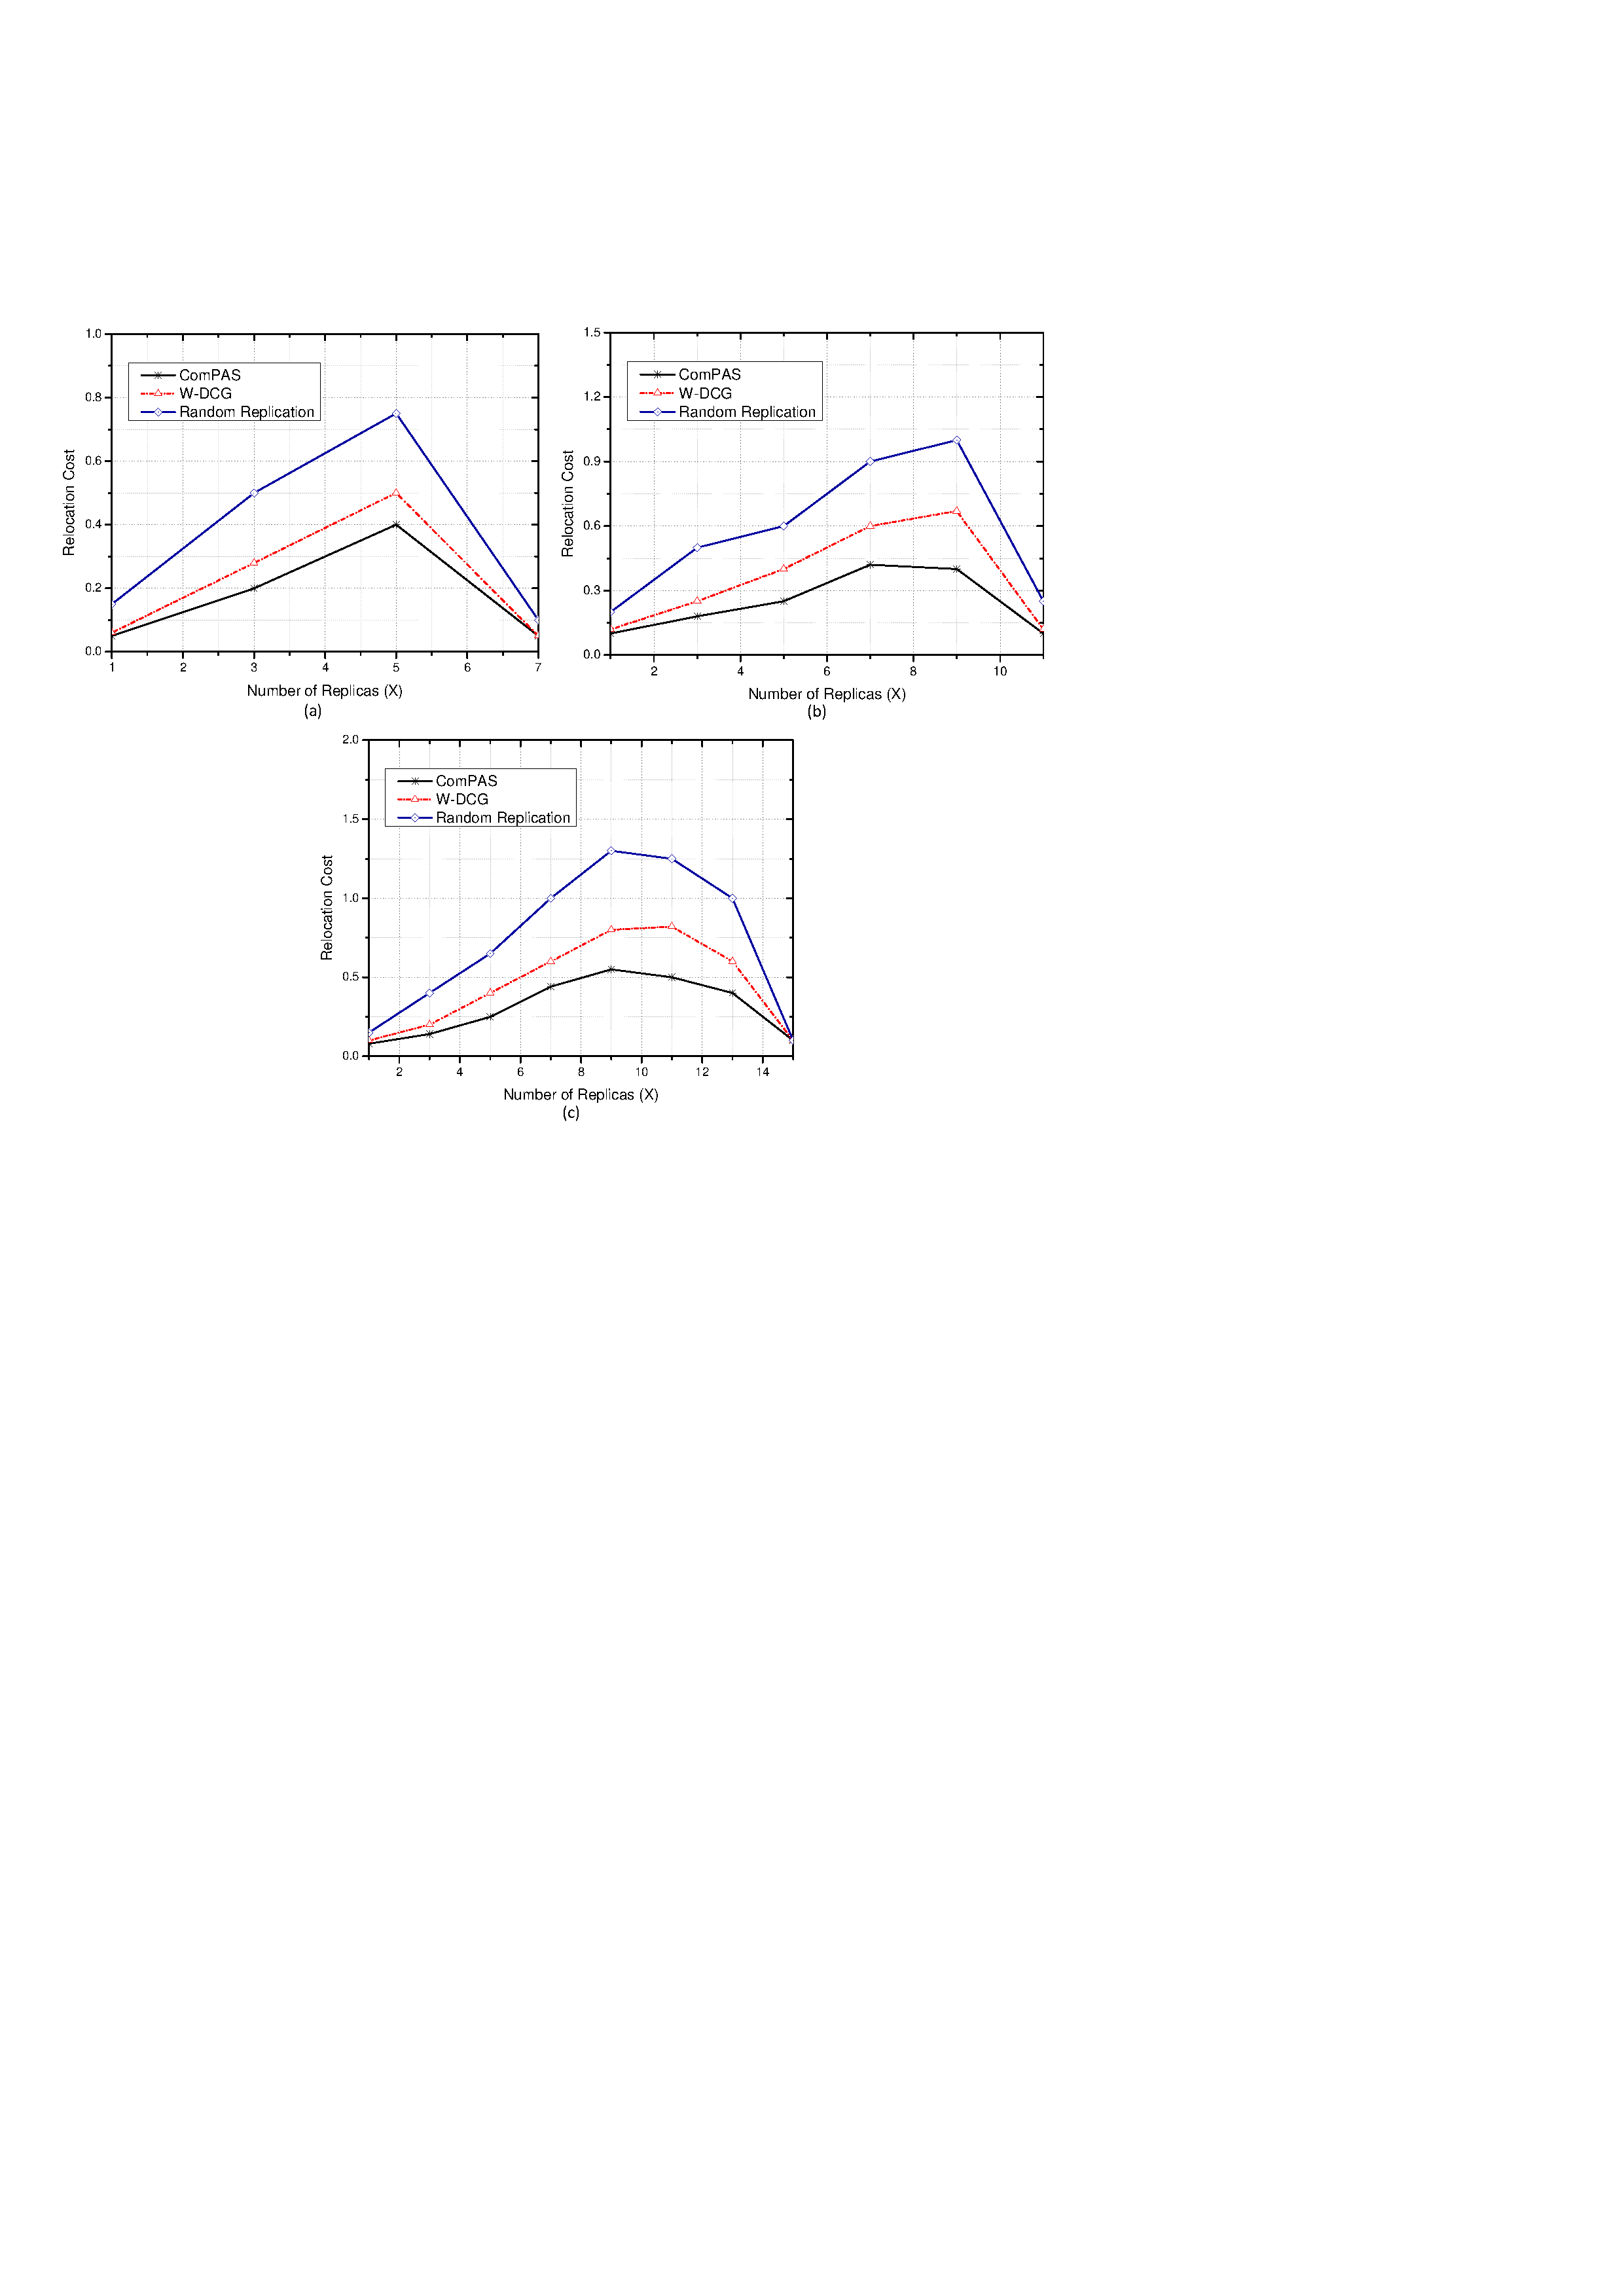
\includegraphics[width=0.95\textwidth]{Chap4-Ev-Fig3.pdf}
  \end{tabular}
  \caption{Relocation cost for ComPAS, W-DCG and Random replication.}
\end{center}
\end{figure}

Fig. 4.10(b) displays the variation of traffic with varying number of nodes. It is easily visible that as the number of nodes increases, the traffic for ComPAS, W-DCG and random replication also increases because every node broadcasts its properties and as the number of nodes increases groups and then social communities also increase. This results in increasing number of messages for group/community allocation and broadcasting. Traffic is zero for no replication as seen on the graph because it does not replicate data items.

\subsection{Relocation Cost}\label{Chap4_05_03}
\esubsection{Relocation Cost}
Since we want to exploit the social relationship of the network, replica relocation may happen. This property will weaken over time if replicas stay unmoved. On the other hand, if replica relocation happens too often, it results in significant overhead for the system due to communication and processing costs involved. Therefore, a desirable replica allocation method should keep the replica relocation cost as low as possible.

The relocation cost (number of replicas relocated from one storage space to another) for ComPAS, W-DCG and random replication is depicted in Fig. 4.11 for cases $G$=8 (Fig. 4.11(a)), $G$=12 (Fig. 4.11(b)) and $G$=16 (Fig. 4.11(c)). The plots shows that there exists a special value of $X$ where the relocation cost is higher. This is because, when $X$ is closer to the two extreme values (1 and $G$-1), there are too many replicas to relocate (very small $X$) and not enough flexibility for where the replicas can be relocated (very large $X$). In all the graphs (Figs. 4.11(a)-(c)), the relocation cost is small. In Fig. 4.11(a) when there are $G$=8 storage spaces, ComPAS incurs less than 0.4 replicas that need relocation. When the number of storage space $G$=16 (Fig. 4.11(c)), the relocation cost doesn't exceed 0.6 (relocated replicas). Therefore, it is obvious from the evaluation that ComPAS is highly efficient when relocation of replicas happened in the network.

\begin{figure}[h]
\begin{center}
  \begin{tabular}{c}
  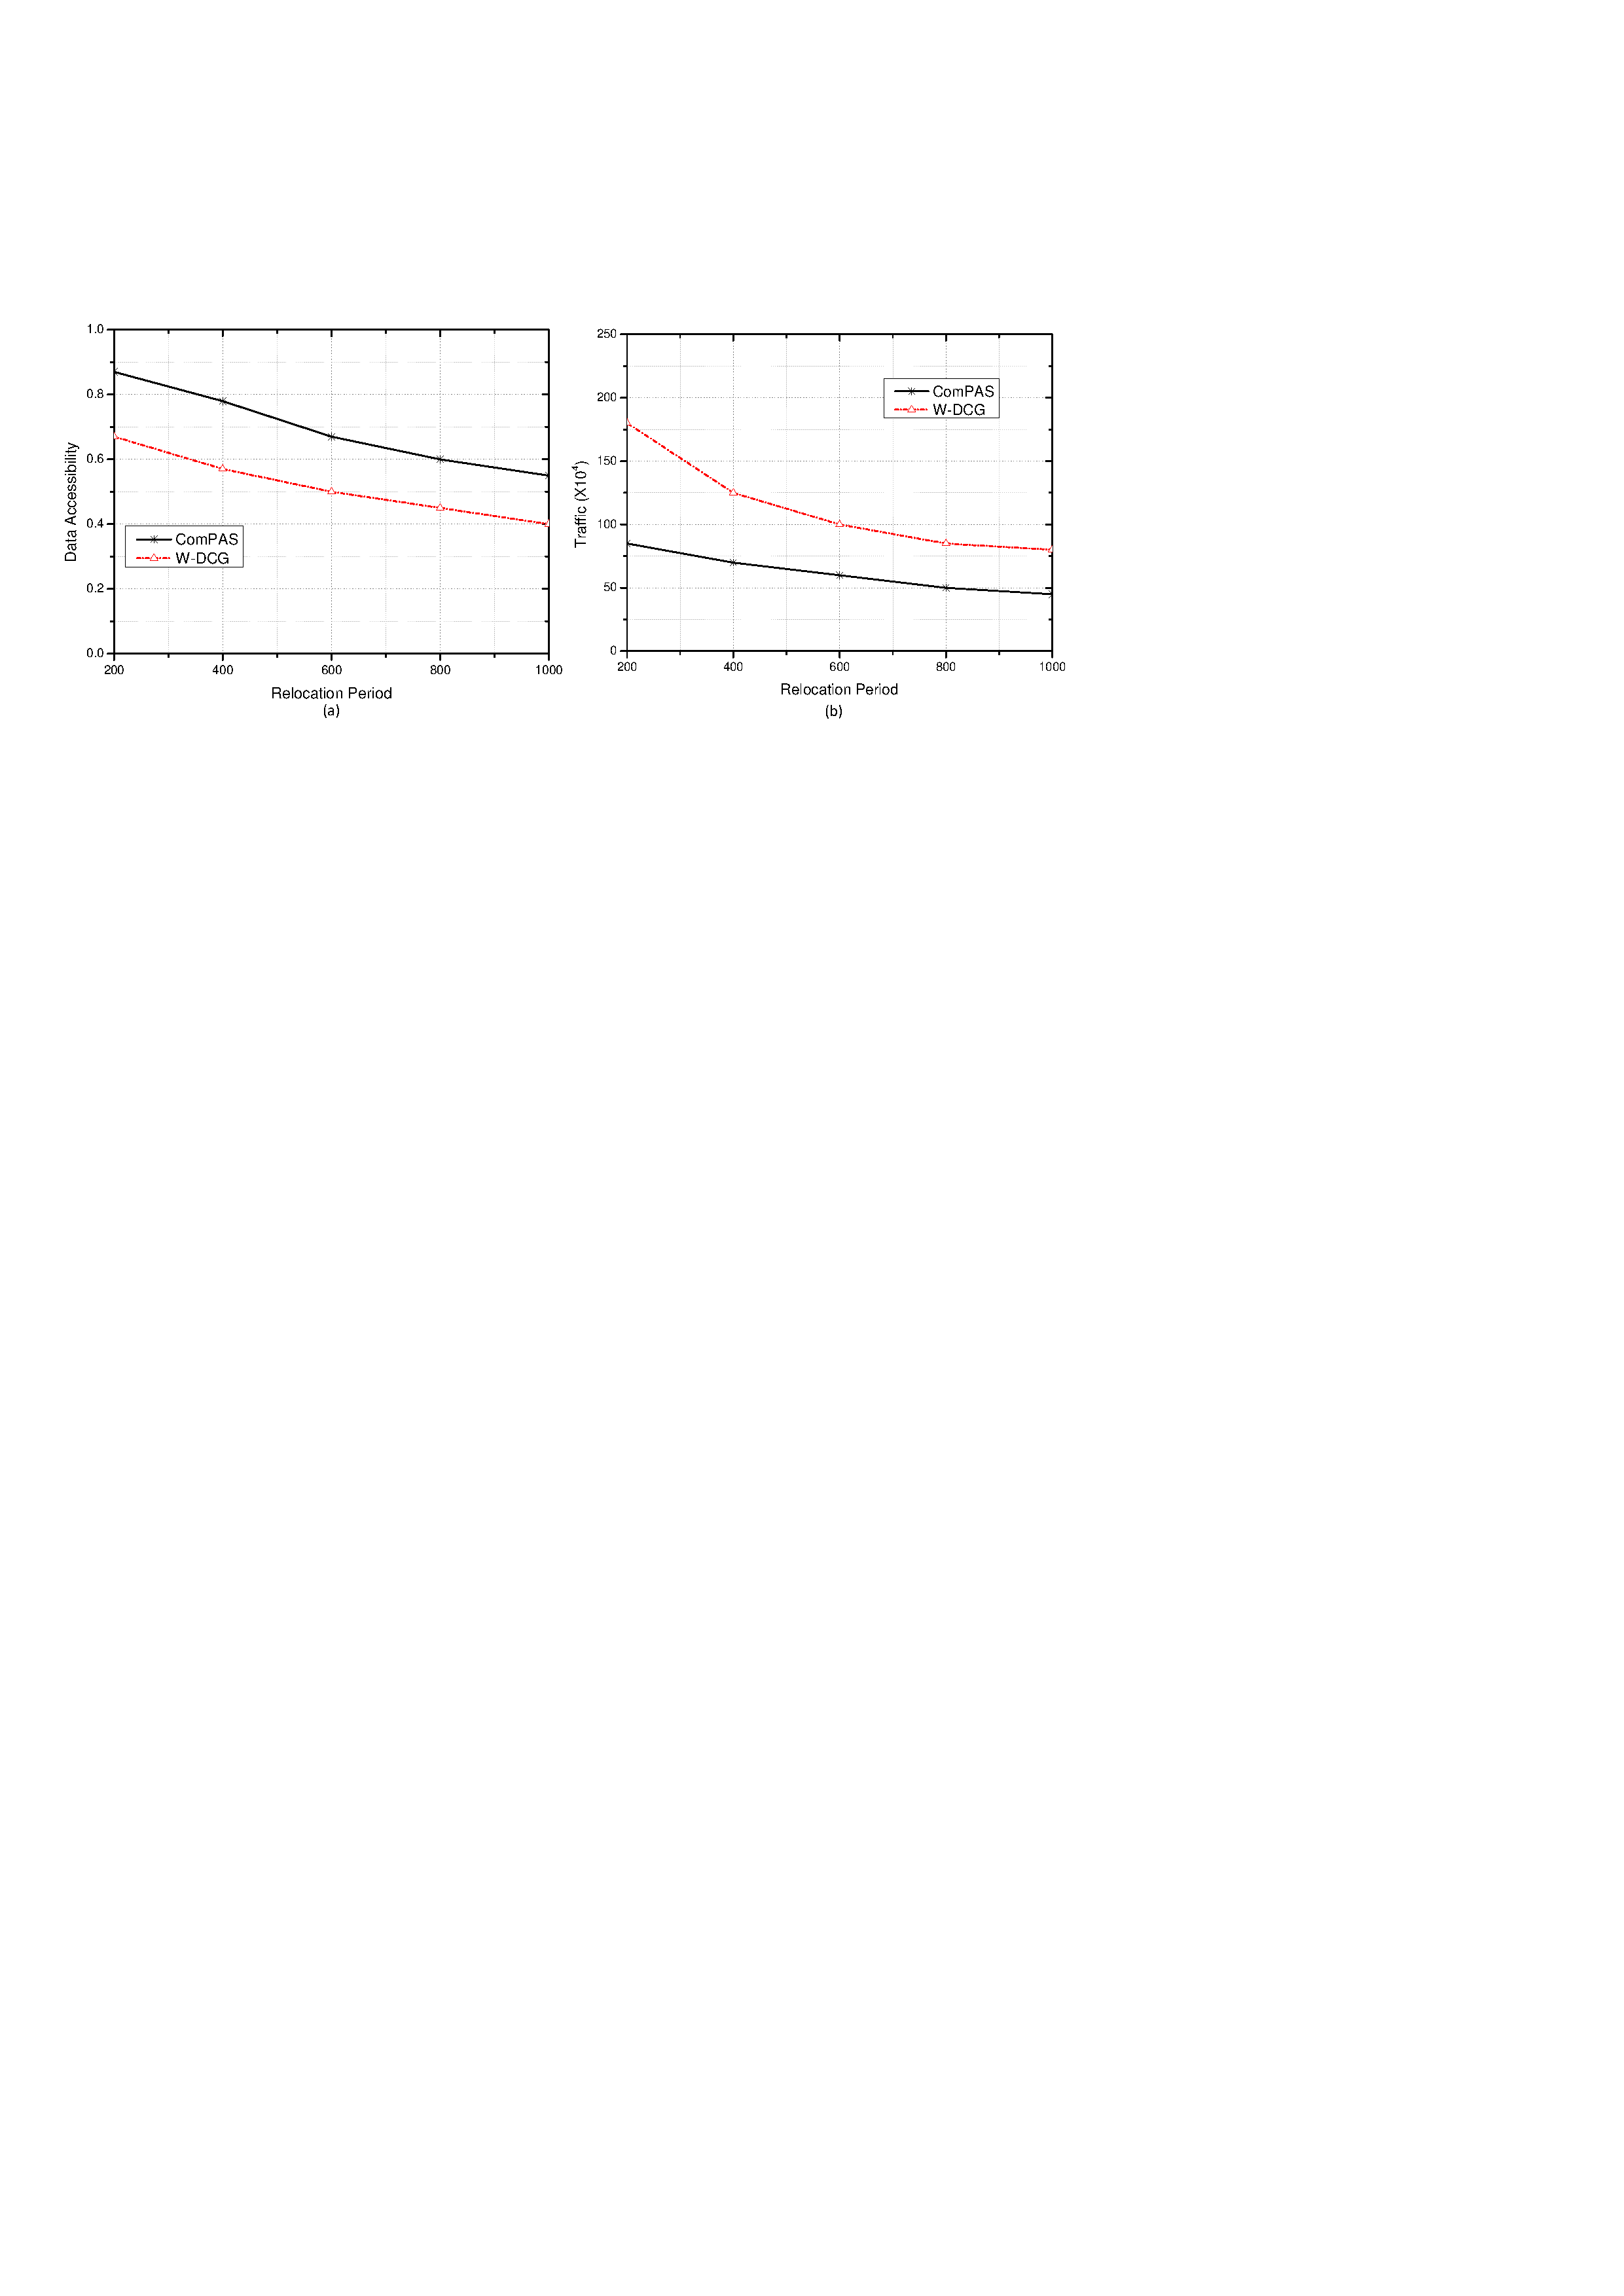
\includegraphics[width=0.95\textwidth]{Chap4-Ev-Fig4.pdf}
  \end{tabular}
  \caption{The effect of relocation period on (a) Data accessibility, and (b) Traffic.}
\end{center}
\end{figure}

Next, we investigate the effect of the varied relocation period in data accessibility and traffic of W-DCG and ComPAS in Figs. 4.12(a) and (b) with the relocation period ranging from 200 to 1000. We observe from Fig. 4.12(a) that the data accessibility increases as relocation period decreases. It can be described that a shorter relocation period shows the more executions of relocation methods and, therefore, makes both replica relocation methods be able to quickly adapt to the mobility behavior of mobile nodes by frequently generating allocation units according to the network connectivity. It's also observed that ComPAS outperforms W-DCG in data accessibility. This result shows the importance of the consideration of group mobility. Therefore, the data accessibility of ComPAS is higher than that of W-DCG. In addition, the performance gain of ComPAS over W-DCG in data accessibility increases as the relocation period decreases. The reason is that each execution of ComPAS can obtain better replica allocations than that of W-DCG and, hence, a short relocation period strengthens the advantage of ComPAS over W-DCG. Fig. 4.12(b) shows the produced network traffic of ComPAS and W-DCG with varied relocation period values. We observe that the produced network traffic increases as the relocation period decreases. The reason is that with the same time interval, a shorter relocation period indicates more executions of the relocation methods and, hence, implies more exchanged messages. It is also shown that the produced network traffic of ComPAS is smaller than that of W-DCG.


\subsection{Number of Mobility Groups}\label{Chap4_05_04}
\esubsection{Number of Mobility Groups}
\begin{figure}[h]
\begin{center}
  \begin{tabular}{c}
  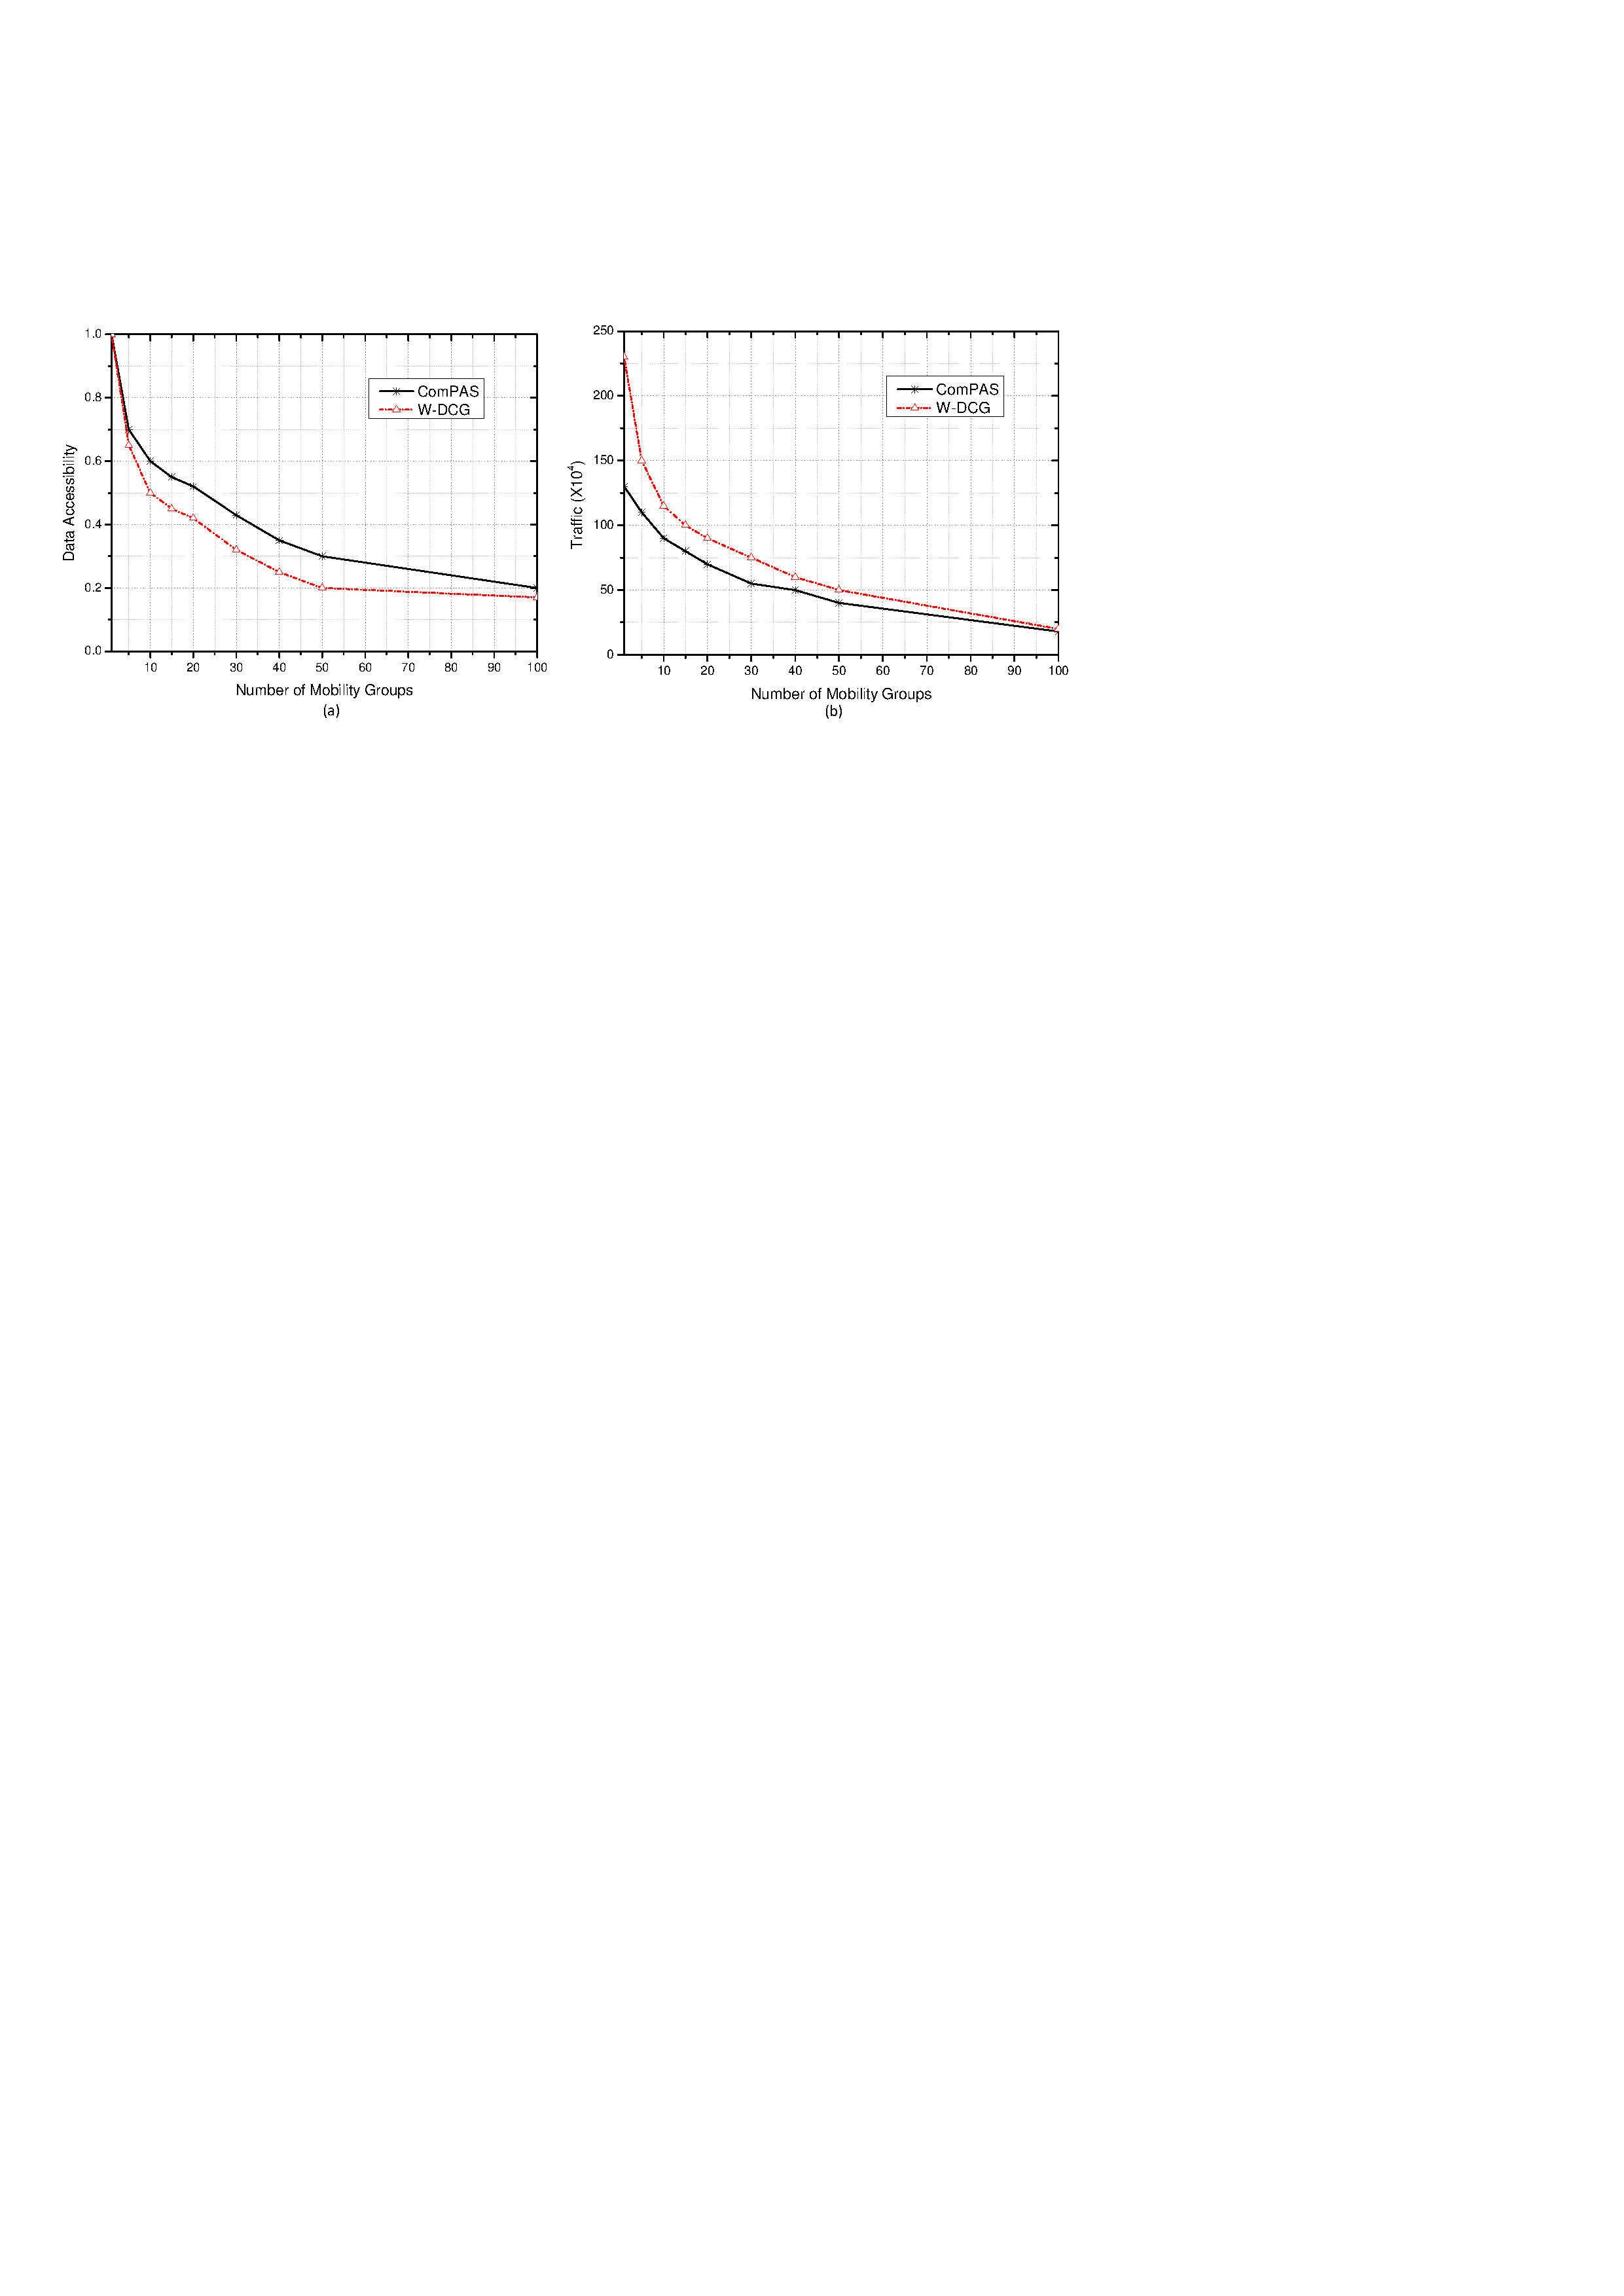
\includegraphics[width=0.95\textwidth]{Chap4-Ev-Fig5.pdf}
  \end{tabular}
  \caption{The effect of the number of mobility groups on (a) Data accessibility, and (b) Traffic.}
\end{center}
\end{figure}

The effects in data accessibility and traffic for both methods with varied number of mobility groups are shown in Figs. 4.13(a) and (b). The number of mobility groups is set from 1 to 100. The graph shows that the data accessibilities of ComPAS and W-DCG are equal to 100\% when the number of groups is set to one. In the case with one mobility group, the data accessibility is dependent on the initial network connectivity. In this evaluation, since the initial network topology is connected, the network topology will not be partitioned and all mobile nodes are connected throughout the simulation, thereby having complete data accessibilities for both methods. When the number of groups is set to 5, the data accessibilities are reduced to around 60\%. These results show that the data accessibilities of ComPAS and W-DCG are similar when the number of mobility groups is small. When the number of mobility groups is larger than five, the data accessibilities of both methods decrease as the number of mobility groups increases. It is because that with the same number of mobile nodes, the smaller number of mobile groups indicates that more mobile nodes are of similar moving behavior. Hence, more mobile nodes can share their storage by constructing large allocation units and, hence, increase the data accessibility.

Moreover, as shown in Fig. 4.13(a), ComPAS outperforms W-DCG especially when the number of mobility groups is large (from 10 to 50 in this simulation). The larger number of mobility groups indicates that the movement behaviors of all mobile nodes are less regular. However, the performance gain of ComPAS over W-DCG diminishes greatly when the number of mobility groups is large. Under these cases, since the network topology changes quickly and is highly likely to be partitioned into several disconnected partitions, the effect of replication diminishes significantly. Fig. 4.13(b) shows the amount of traffic produced by both methods increases as the number of mobility groups decreases. When the number of mobility groups is large, ASNET tends to be separated into many disconnected partitions since fewer mobile nodes are of similar moving behavior. Therefore, the amount of produced traffic of both methods is small since many mobile nodes disconnect with others when the ASNET is separated into several partitions.

\subsection{Efficiency of Replica Allocation Consistency}\label{Chap4_05_05}
\esubsection{Efficiency of Replica Allocation Consistency}
\begin{figure}[h]
\begin{center}
  \begin{tabular}{c}
  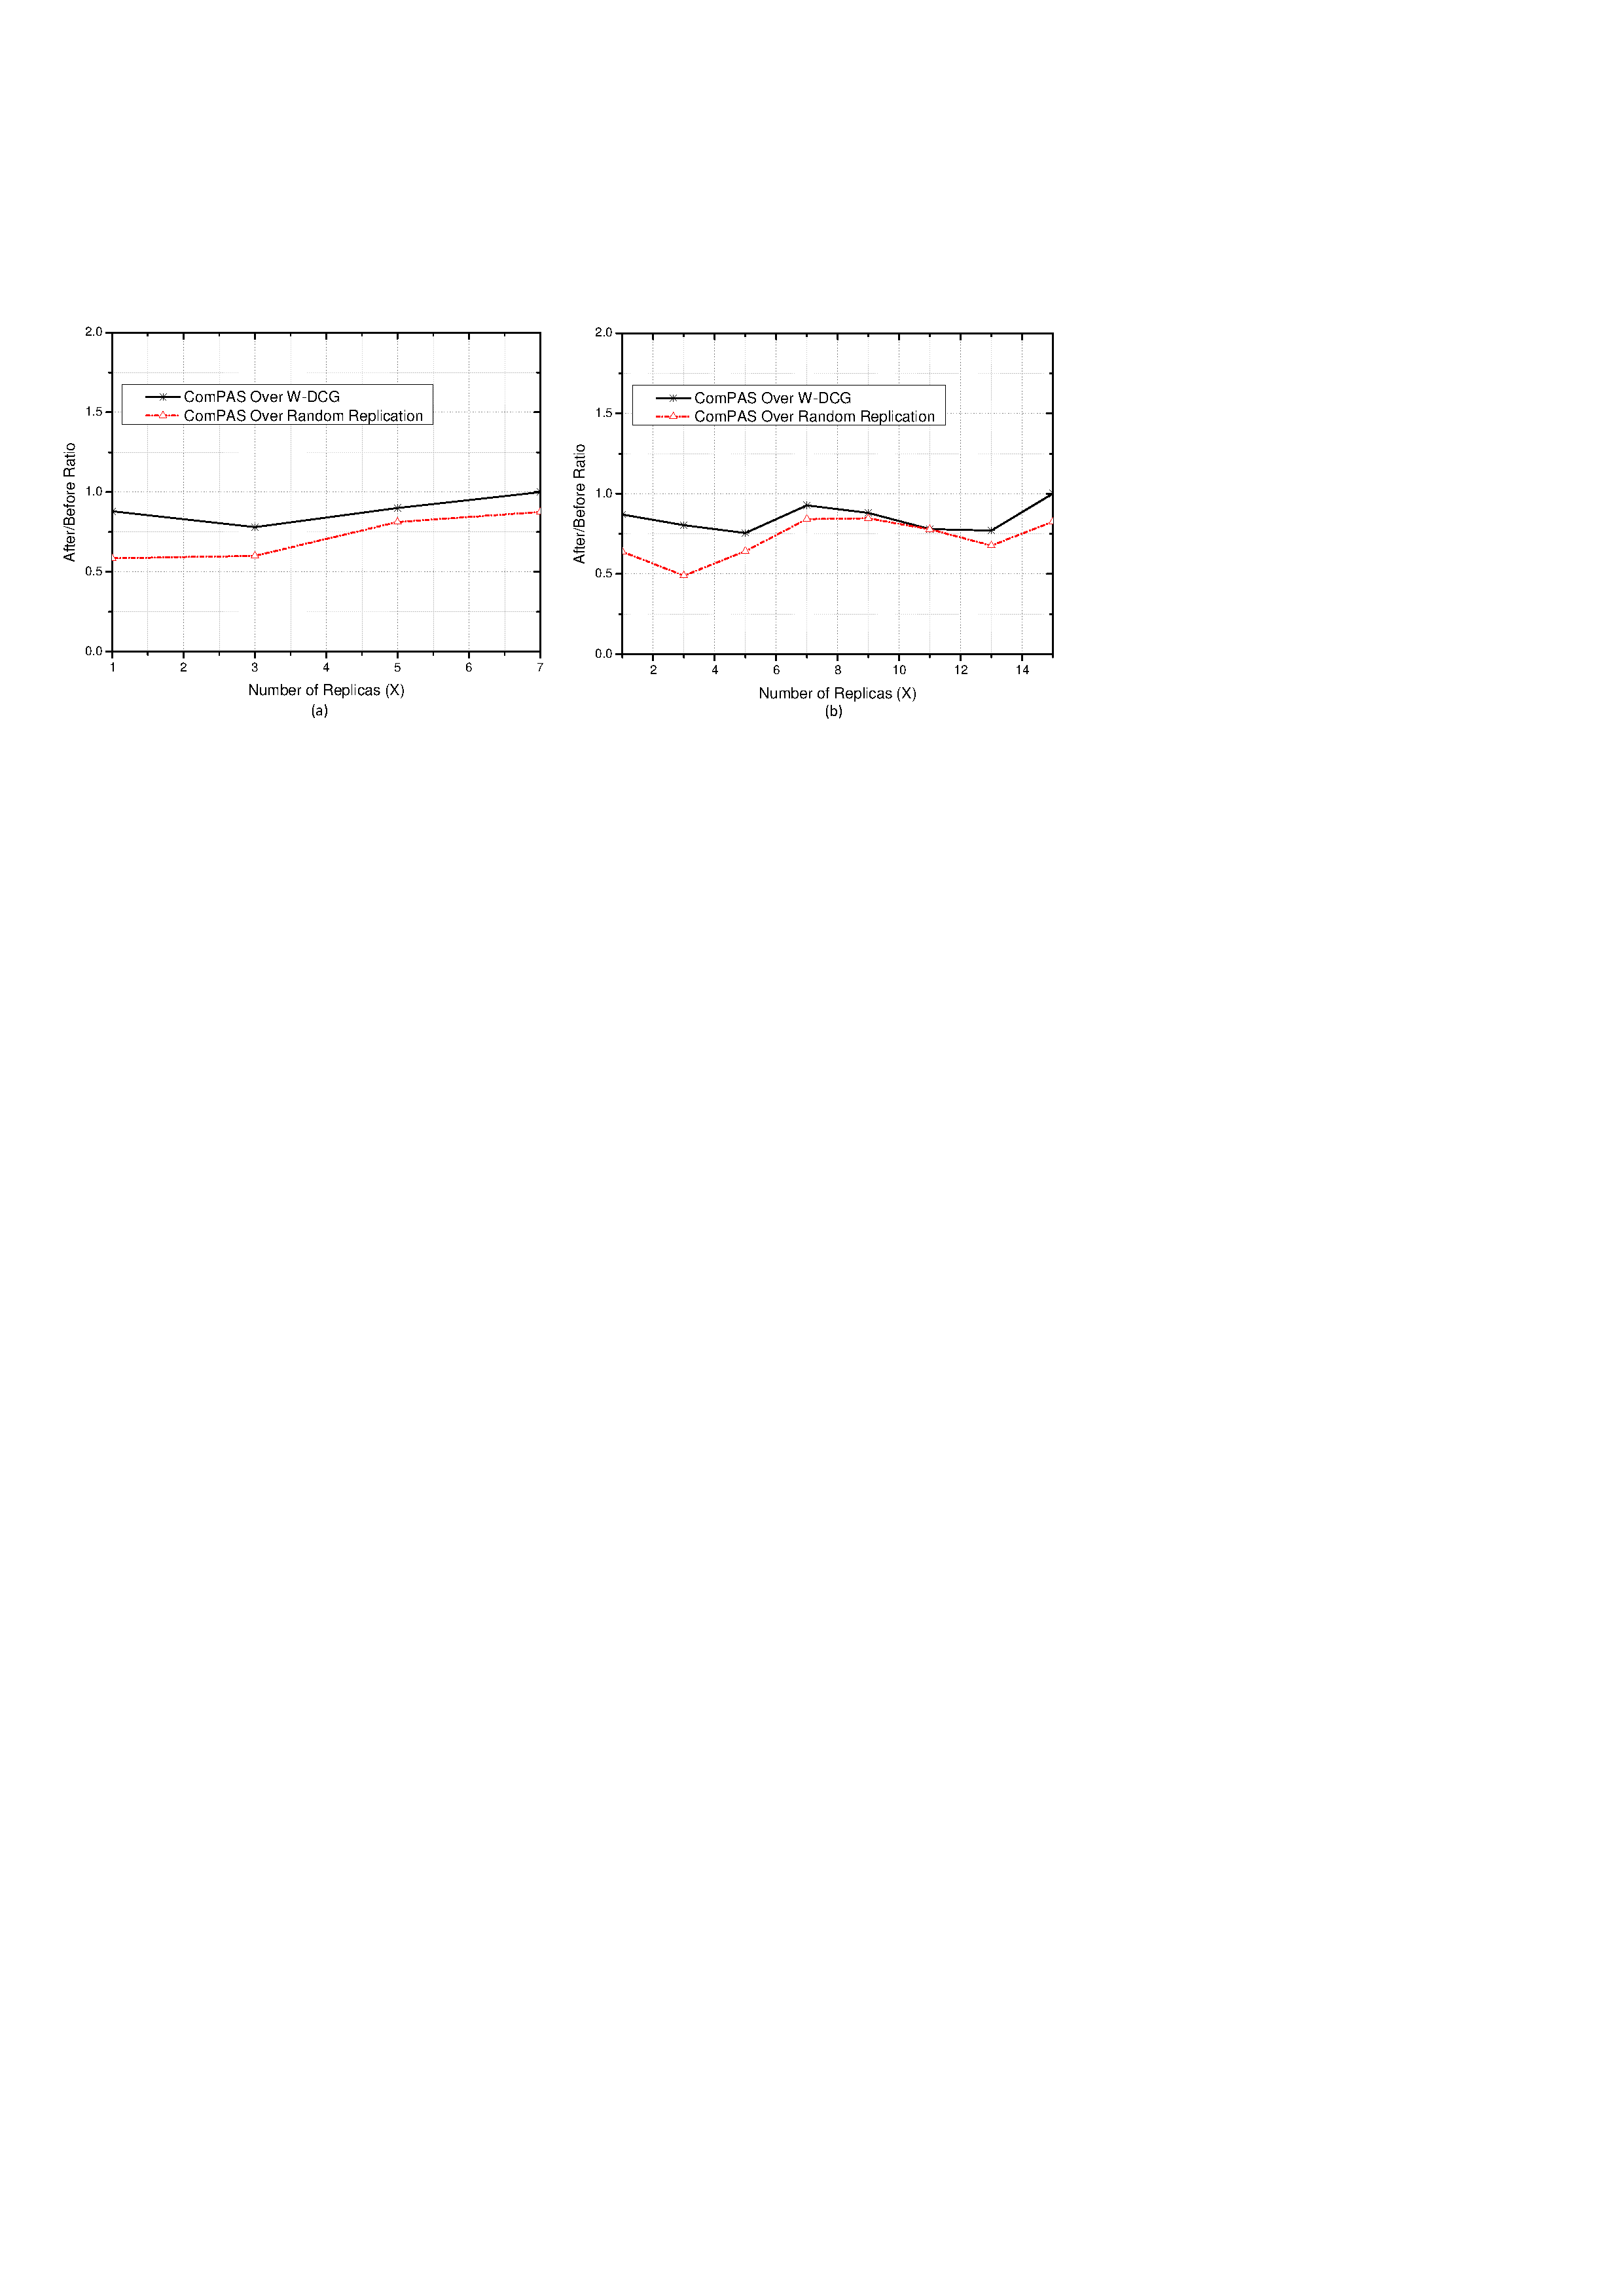
\includegraphics[width=0.95\textwidth]{Chap4-Ev-Fig6.pdf}
  \end{tabular}
  \caption{Consistency of ComPAS replica allocation efficiency over W-DCG and random replication for cases (a) $G$=8 storage space and (b) $G$=16 storage space.}
\end{center}
\end{figure}

To further validate the performance of our proposed replica allocation scheme, we have also performed an evaluation to measure the consistency of ComPAS's superiority to W-DCG and random replication in terms of replica allocation efficiency. We compute a measure called "after/before ratio" which is the ratio a/b where a is the improvement ratio of ComPAS over W-DCG and random replication after the relocation (relocation cost) and b is the ratio before relocation (read cost). The evaluation result is plotted in Figs. 4.14(a) and (b) for $G$=8 and $G$=16, respectively. For both cases, the ratio is consistent between 0.5 and 1. This implies that ComPAS is constantly superior to W-DCG and random replication. Besides, increase in the number of relocated replicas and storage spaces in the social graph can't have a negative impact on the effectiveness and consistency of ComPAS. Even at a higher number of nodes, replicas ($X$) and storage space ($G$) than our evaluation environment, it is evident that the efficiency and consistency will still be better for ComPAS. Finally, the results confirm the efficiency and consistency of the replica allocation method that we have proposed over W-DCG and random replication.

\section{Summary}\label{Chap4_06}
\esection{Summary}
We have introduced the importance of exploiting social properties and group mobility modeling in the replica allocation of user data for ASNETs. We have specifically proposed ComPAS, a system based on partitioning of social community combined with social relationship and a user level replication so that data availability for all users is guaranteed. The system gives a fixed number of replicas required for each user that results in an efficient replication solution. The efficiency of the proposed method is better compared to W-DCG, and by a large margin compared to random replication scheme, as shown in our evaluation and analysis. We showed that ComPAS offers significant gains in data availability, efficiency and consistency while reducing traffic and relocation cost.
